\documentclass[11pt]{article}
\usepackage[a4paper,margin=0.82in]{geometry}
\usepackage{microtype}
\usepackage{graphicx}
\usepackage{booktabs}
\usepackage{tabularx}
\usepackage{array}
\usepackage{ragged2e}
\usepackage{adjustbox}
\usepackage{float}
\usepackage{placeins}
\usepackage{caption}
\usepackage{amsmath}
\usepackage{amssymb}
\usepackage{xcolor}
\usepackage{hyperref}
\usepackage{fancyhdr}
\usepackage{enumitem}
\usepackage{listings}
\usepackage{url}
\hypersetup{colorlinks=true,linkcolor=blue,citecolor=blue,urlcolor=blue}
\graphicspath{{assets/}}
\definecolor{codegray}{RGB}{245,247,250}
\definecolor{deepteal}{RGB}{15,118,110}
\newcolumntype{Y}{>{\RaggedRight\arraybackslash}X}
\captionsetup{font=small,labelfont=bf}
\lstset{
  backgroundcolor=\color{codegray},
  basicstyle=\ttfamily\footnotesize,
  breaklines=true,
  frame=single,
  columns=fullflexible,
  keepspaces=true
}
\pagestyle{fancy}
\fancyhf{}
\fancyhead[L]{\small Agentic Research \& Decision Intelligence Platform}
\fancyhead[R]{\small Final Project Report}
\fancyfoot[C]{\thepage}
\setlength{\headheight}{14pt}
\setlist[itemize]{leftmargin=1.2em,itemsep=0.25em}
\setlength{\parskip}{0.45em}
\setlength{\parindent}{0pt}
\emergencystretch=2em

\title{\textbf{Agentic Research \& Decision Intelligence Platform}\\\large Robust Multi-Agent Research Workflow with Evidence, Algorithms, Formulas, UI Artifacts, and Reproducible Evaluation}
\author{Final Course Project}
\date{\today}

\begin{document}
\maketitle

\begin{abstract}
This report presents a complete multi-agent research and decision-intelligence platform. The system converts one high-level topic into a reproducible research workflow: planning, evidence retrieval, structured analysis, critique, fact-checking, visualization, report generation, evaluation, presentation export, and persistent memory. The report intentionally includes the mathematical scoring formulation, conditional-routing algorithm, implementation tables, generated architecture figures, UI screenshots, and export artifacts. The default demonstration uses deterministic mock mode so that the project can be graded without paid API keys while remaining extensible to live retrieval and model providers.
\end{abstract}

\tableofcontents
\listoffigures
\listoftables
\newpage

\section{Executive Summary}
This final report documents an inspectable agentic research platform, not a single chatbot response. The analyzed run used the topic \textit{Multi-agent AI systems for trustworthy clinical decision support}, operated in Deterministic mock/offline mode, retrieved 21 evidence items, generated 14 visual artifacts, and achieved an evaluation score of 93.1/100 with confidence 95.5/100. The main engineering contribution is a transparent workflow in which planning, retrieval, analysis, critique, fact checking, visualization, reporting, evaluation, presentation, and memory are separate stages with explicit state.

\section{Research Question and Scope}
The project asks whether a graph-based multi-agent system can produce a more trustworthy research artifact than a one-shot prompt. The scope is a university-grade prototype for evidence-grounded research and decision support, demonstrated on trustworthy clinical decision support. It is not a medical device and it does not provide patient-specific recommendations. The deliverable scope includes runnable code, a Streamlit panel, FastAPI endpoints, SQLite memory, generated figures, Markdown/LaTeX/PDF reports, evaluation output, and presentation material.

\section{Background and Related Work}
Retrieval-augmented generation connects model output to external evidence \cite{lewis_2020_rag}. ReAct-style agents combine reasoning and tool use \cite{yao_2022_react}, while Reflexion and Self-Refine demonstrate iterative critique and revision \cite{shinn_2023_reflexion}, \cite{madaan_2023_self_refine}. Evaluation methods for RAG emphasize faithfulness, relevance, and context use \cite{es_2023_ragas}. Clinical decision support research stresses workflow fit, safety, and governance \cite{sutton_2020_cdss}, while hallucination surveys show why fluent text alone is not enough \cite{ji_2023_hallucination_survey}.

\section{System Requirements}
The platform is designed around six requirements. First, the default path must be reproducible without paid API keys. Second, each agent decision must be inspectable through typed state. Third, retrieved evidence and claim checks must be visible. Fourth, tables and figures must compile cleanly into LaTeX without overlapping text or distorted images. Fifth, the UI must expose intermediate and final artifacts for live grading. Sixth, scripts and tests must regenerate the report and screenshots from source.

\section{System Architecture}
The platform has five layers: Streamlit and FastAPI interfaces, graph orchestration, specialized agents, deterministic tools, and persistence/export storage. The figures below are included with constrained width, constrained height, and \texttt{keepaspectratio} so page layout remains stable.


\begin{figure}[!htbp]
\centering
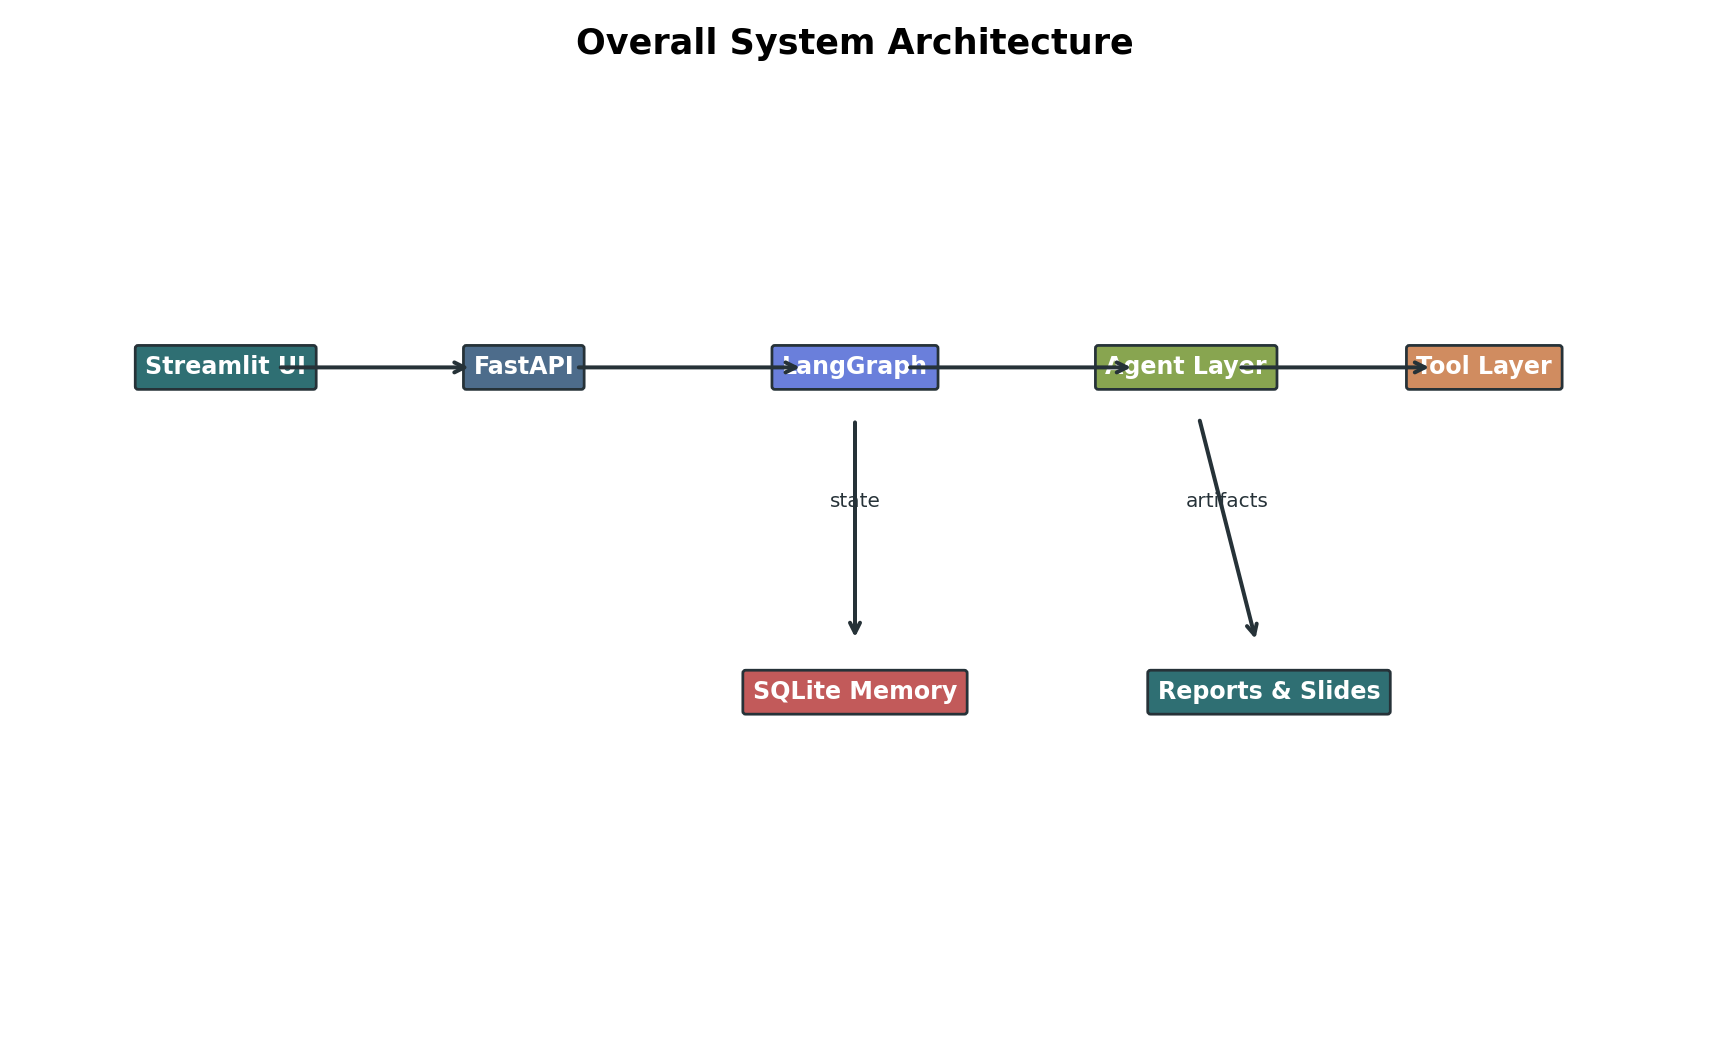
\includegraphics[width=0.96\linewidth,height=0.78\textheight,keepaspectratio]{assets/overall_system_architecture.png}
\caption{System architecture connecting UI, API, graph orchestration, specialized agents, tools, memory, and exported artifacts.}
\label{fig:overall-architecture}
\end{figure}
\FloatBarrier


\begin{figure}[!htbp]
\centering
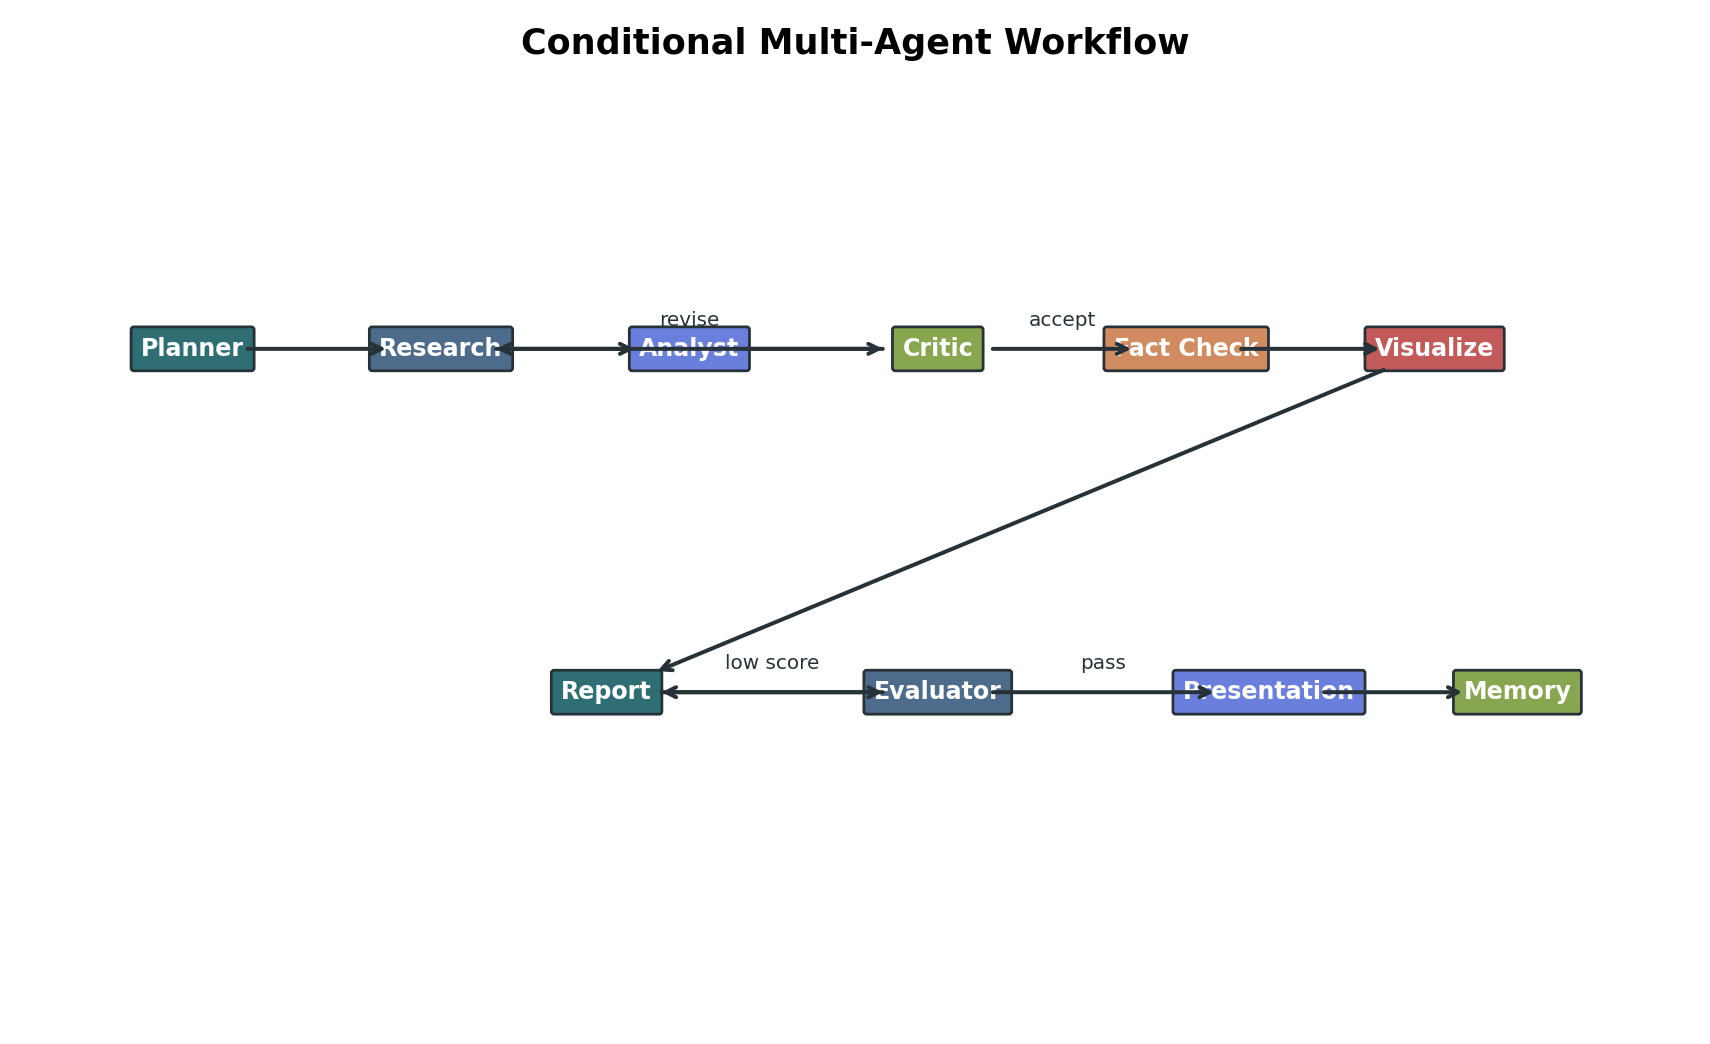
\includegraphics[width=0.96\linewidth,height=0.78\textheight,keepaspectratio]{assets/multi_agent_workflow_diagram.png}
\caption{Conditional multi-agent workflow showing planning, retrieval, analysis, critique, fact-checking, report generation, evaluation, presentation, and memory.}
\label{fig:workflow}
\end{figure}
\FloatBarrier


\begin{figure}[!htbp]
\centering
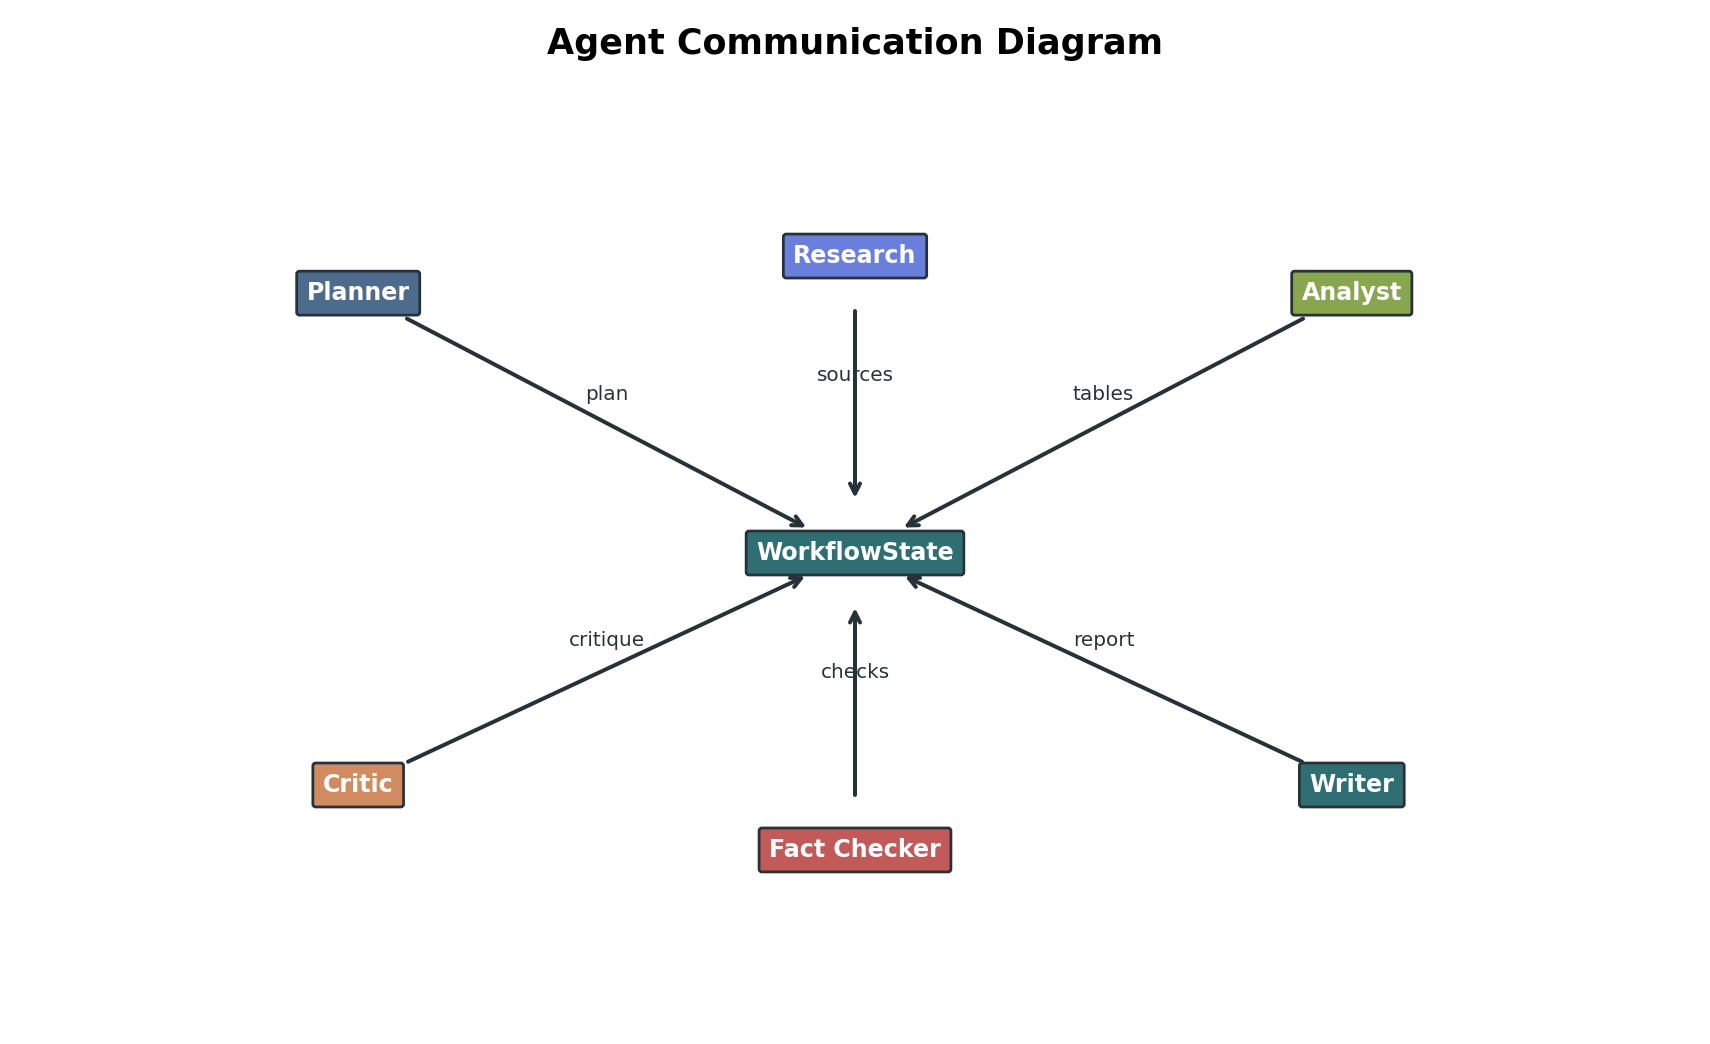
\includegraphics[width=0.96\linewidth,height=0.78\textheight,keepaspectratio]{assets/agent_communication_diagram.png}
\caption{Agent communication through explicit shared WorkflowState fields rather than hidden ad-hoc messages.}
\label{fig:communication}
\end{figure}
\FloatBarrier


\begin{figure}[!htbp]
\centering
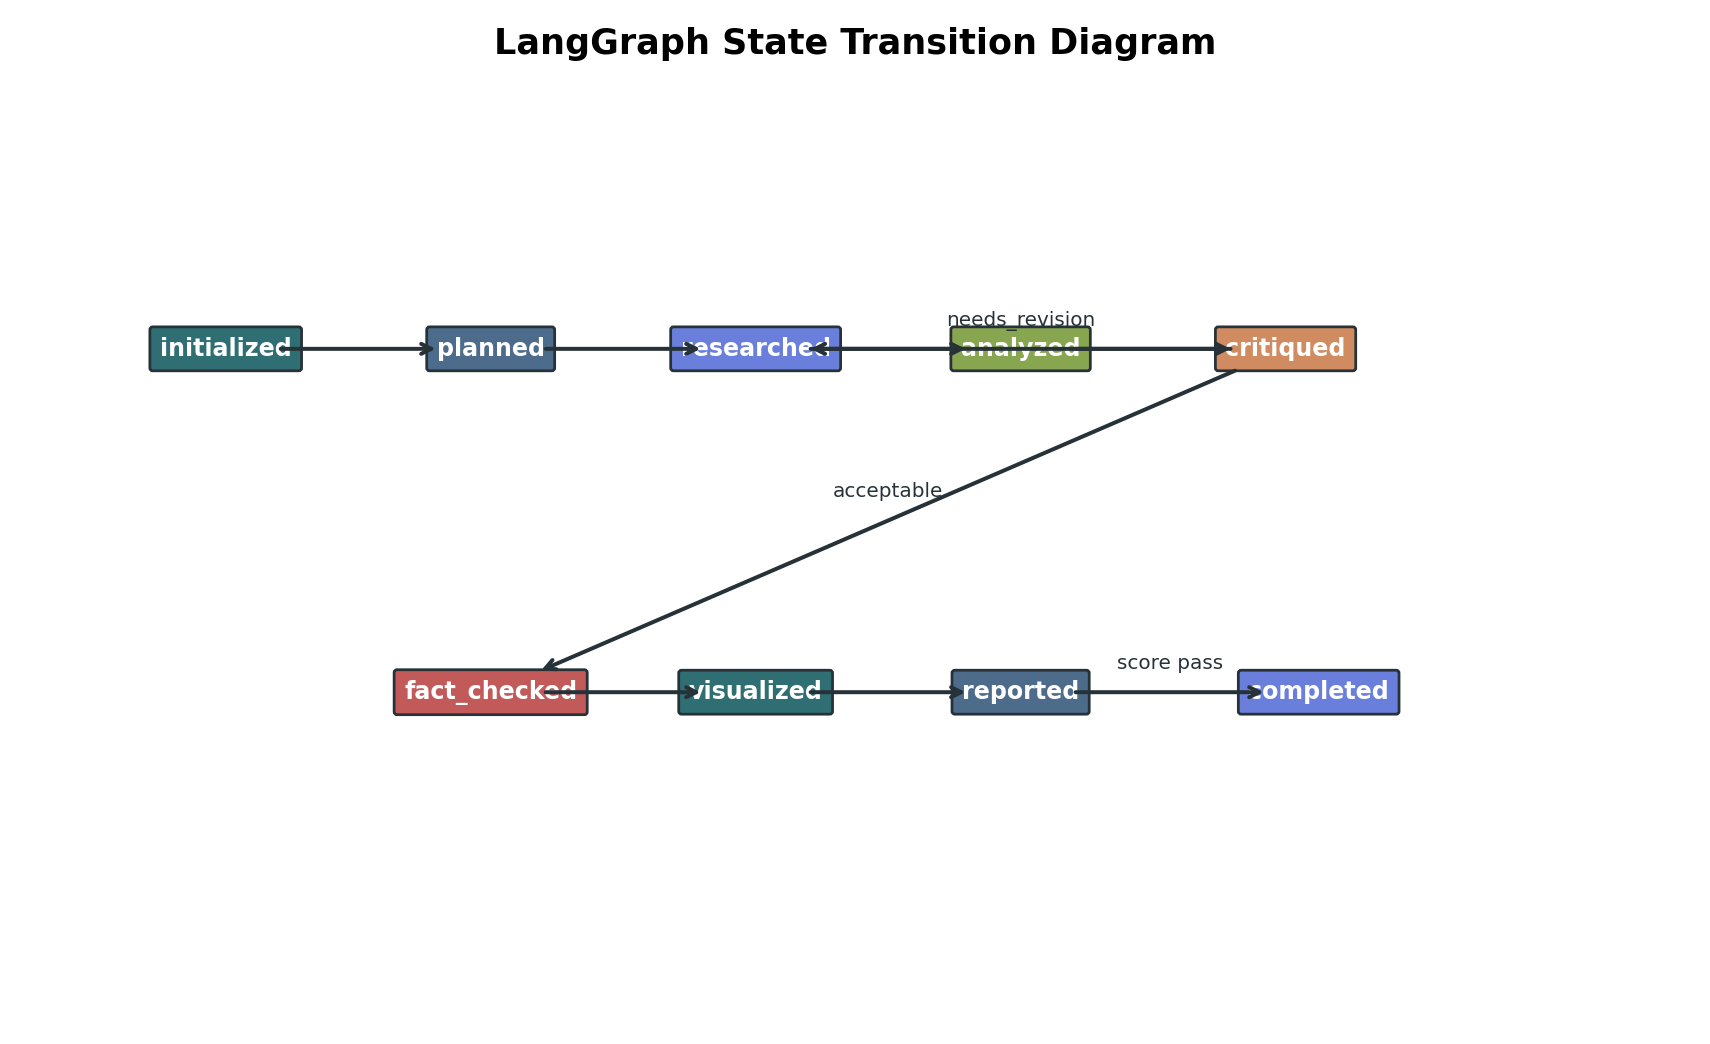
\includegraphics[width=0.96\linewidth,height=0.78\textheight,keepaspectratio]{assets/langgraph_state_transition_diagram.png}
\caption{State transition diagram showing how workflow status values move through the graph.}
\label{fig:state-transition}
\end{figure}
\FloatBarrier


\begin{figure}[!htbp]
\centering
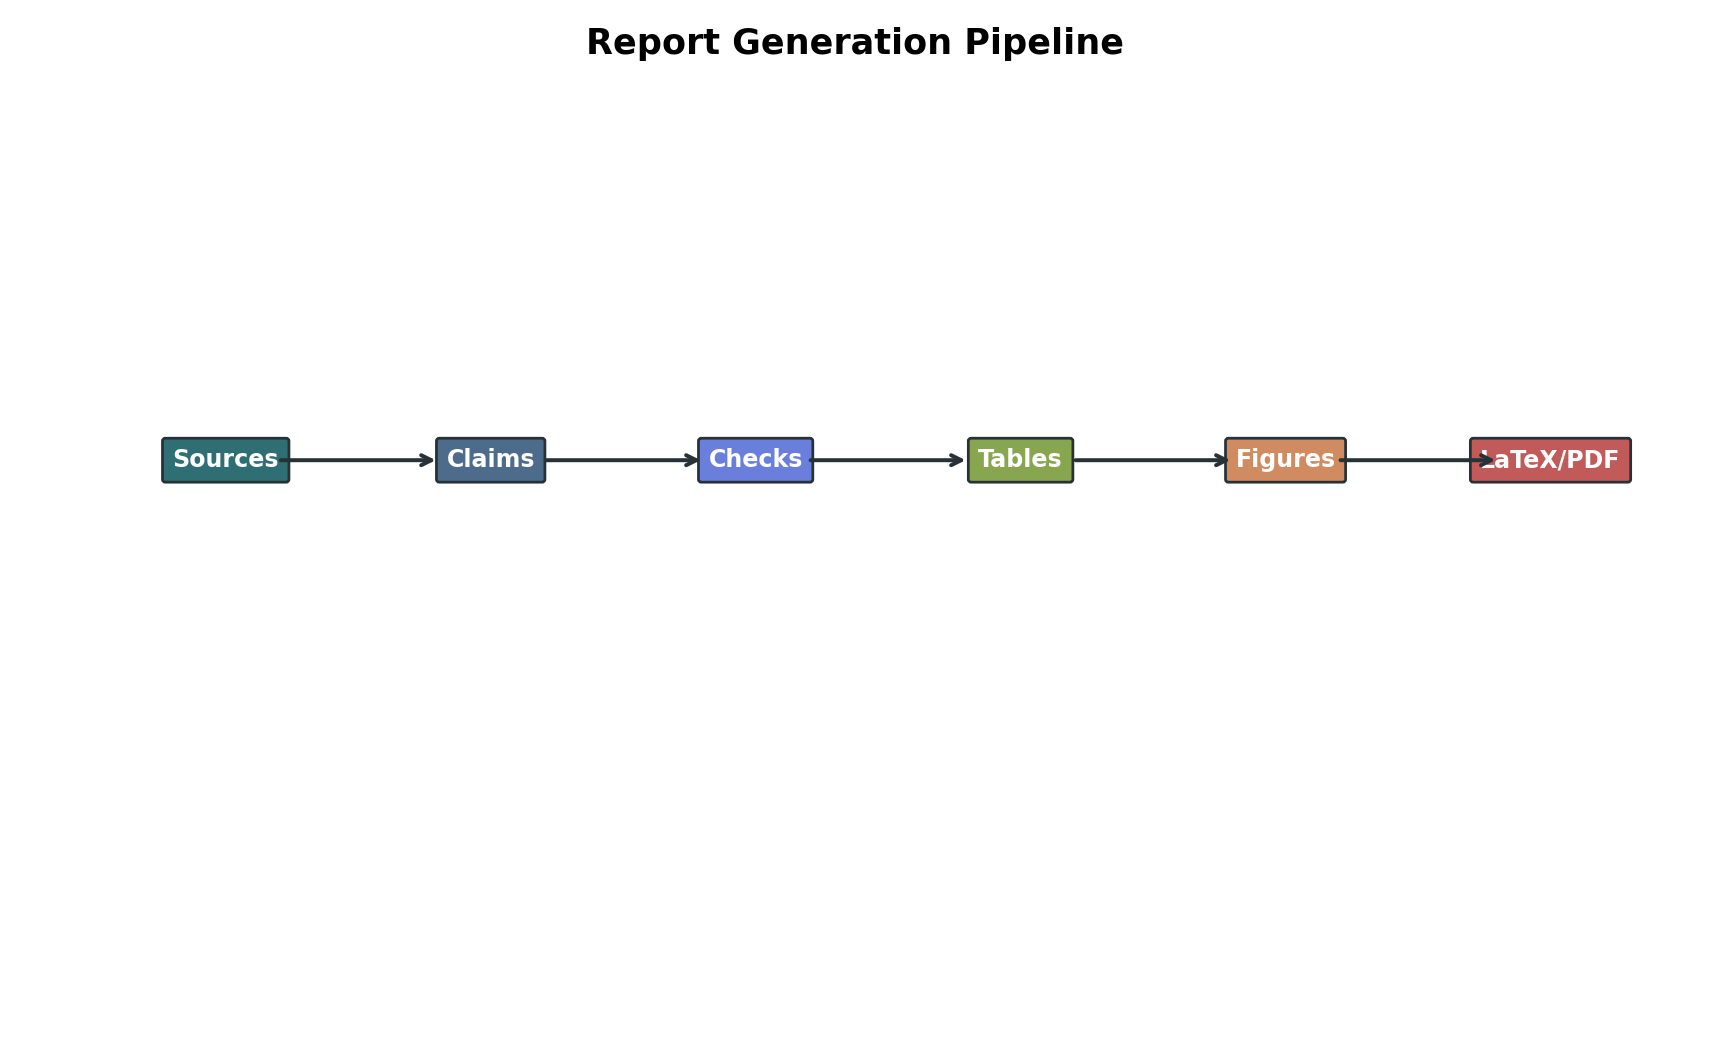
\includegraphics[width=0.96\linewidth,height=0.78\textheight,keepaspectratio]{assets/report_generation_pipeline_diagram.png}
\caption{Report generation pipeline from evidence and tables to Markdown, LaTeX/PDF, presentation, and evaluation outputs.}
\label{fig:report-pipeline}
\end{figure}
\FloatBarrier


\begin{figure}[!htbp]
\centering
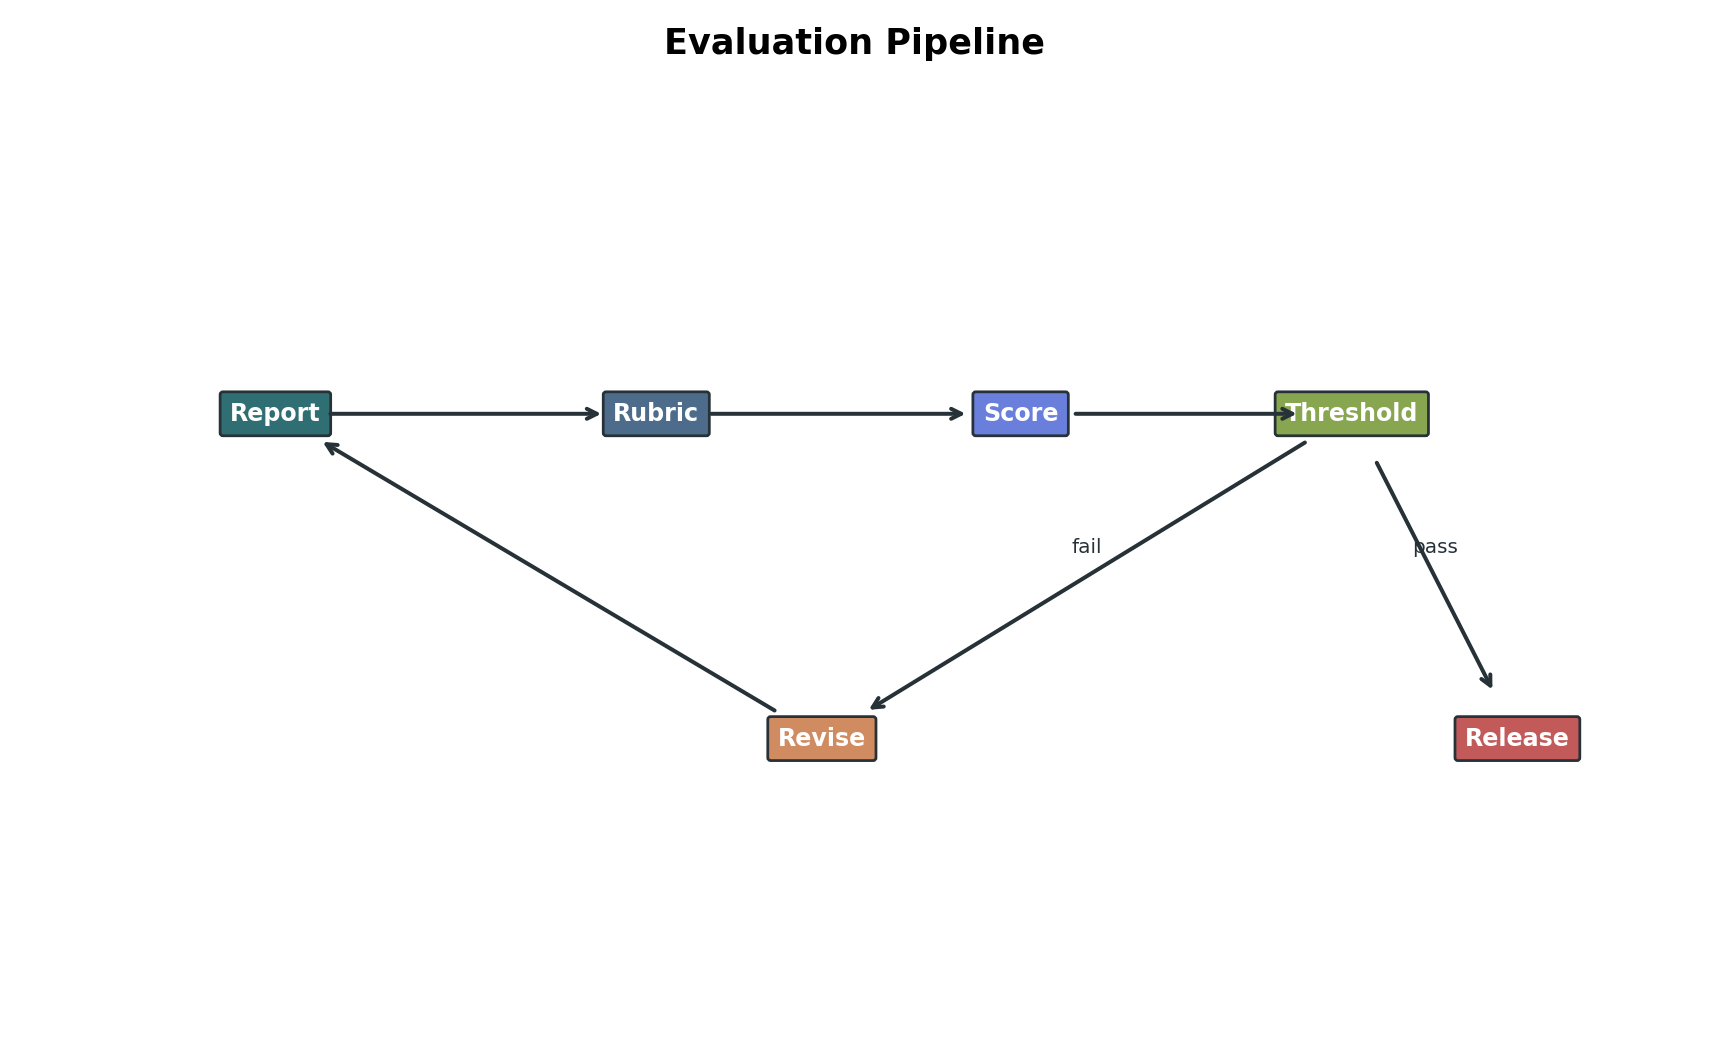
\includegraphics[width=0.96\linewidth,height=0.78\textheight,keepaspectratio]{assets/evaluation_pipeline_diagram.png}
\caption{Evaluation pipeline with rubric scoring, thresholding, and optional revision routing.}
\label{fig:evaluation-pipeline}
\end{figure}
\FloatBarrier


\begin{figure}[!htbp]
\centering
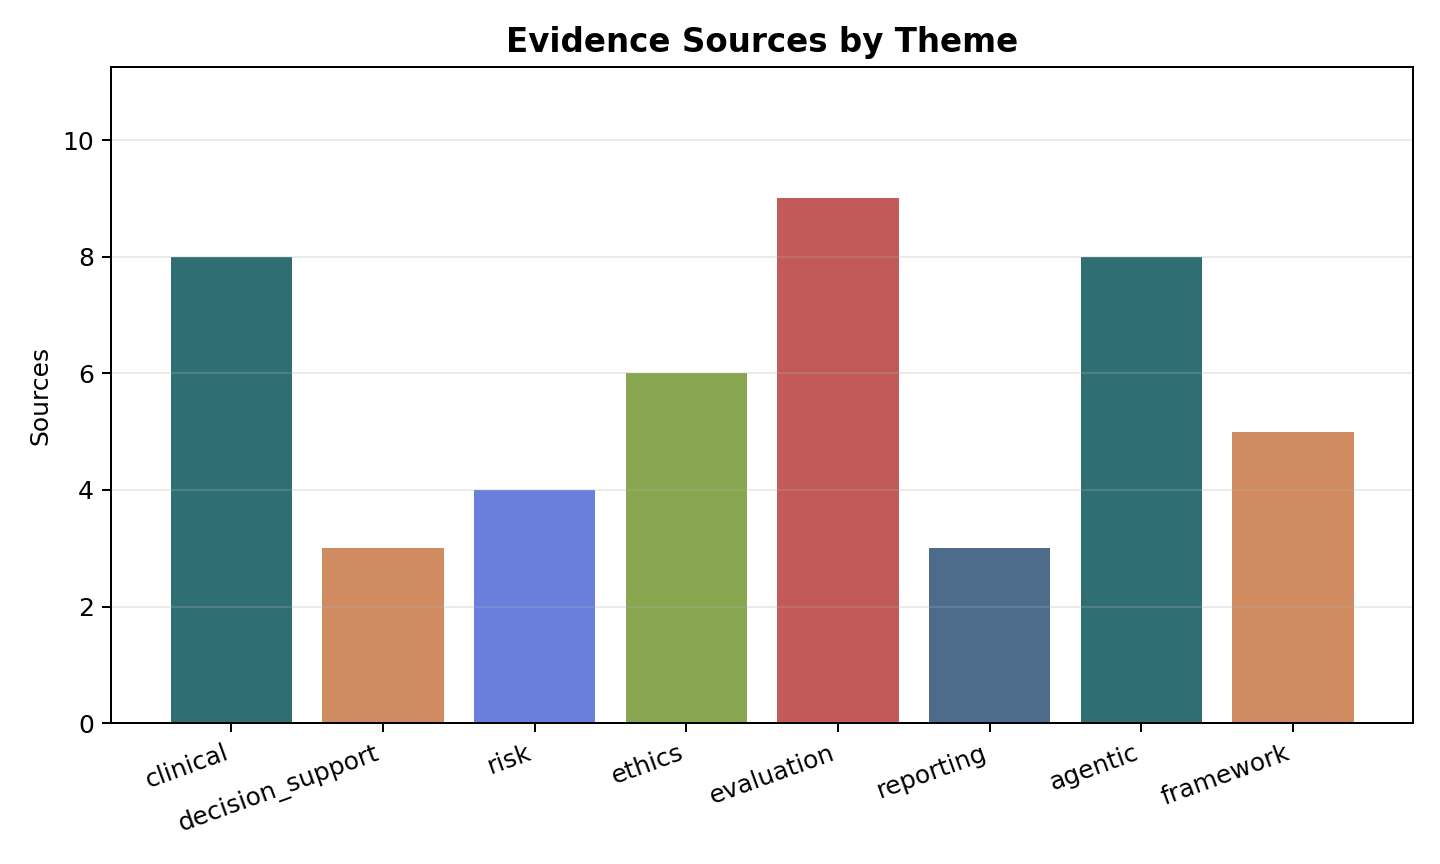
\includegraphics[width=0.96\linewidth,height=0.78\textheight,keepaspectratio]{assets/evidence_by_theme.png}
\caption{Evidence distribution by theme for the deterministic demonstration corpus.}
\label{fig:evidence-theme}
\end{figure}
\FloatBarrier


\begin{figure}[!htbp]
\centering
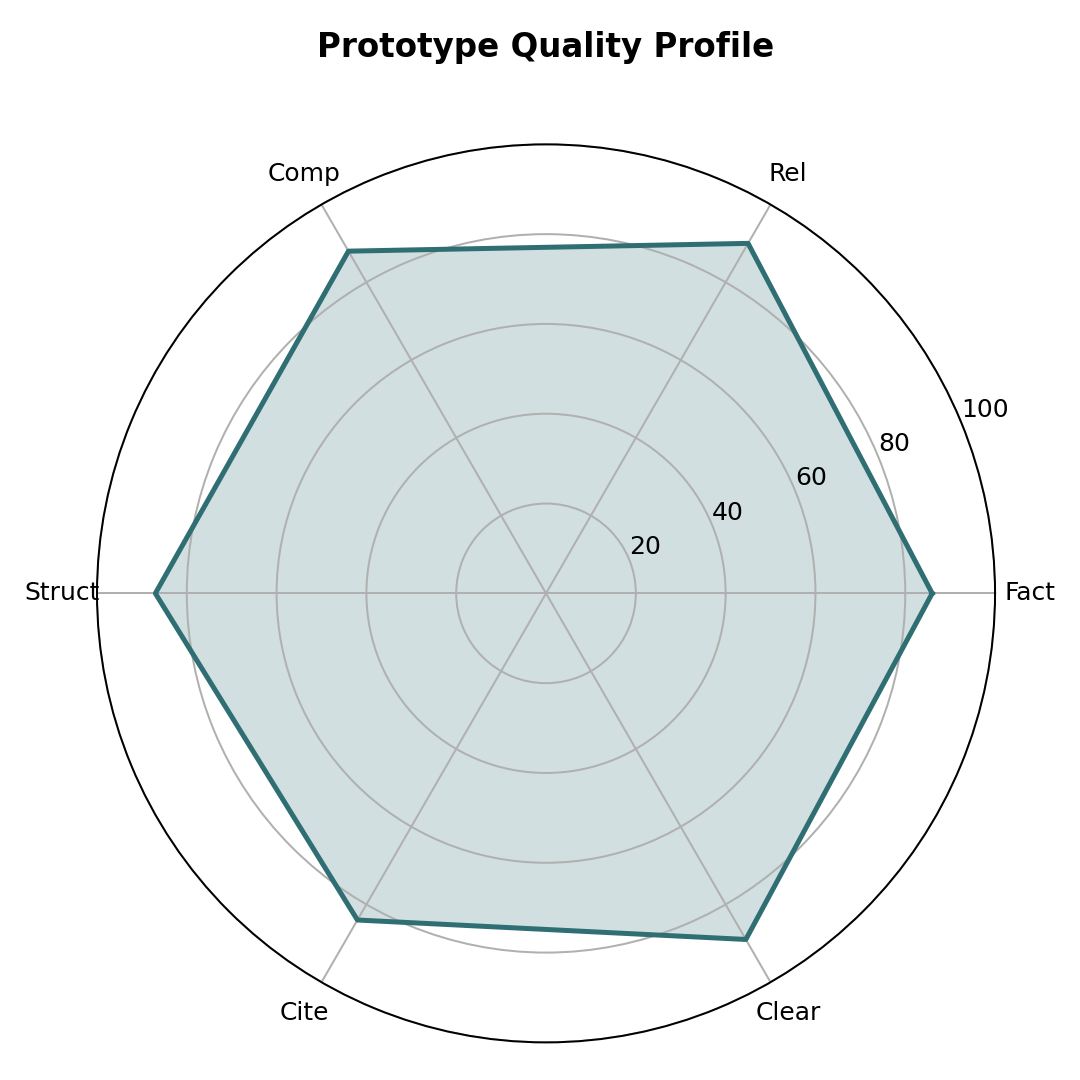
\includegraphics[width=0.96\linewidth,height=0.78\textheight,keepaspectratio]{assets/quality_radar.png}
\caption{Radar chart of selected quality dimensions for the generated artifact.}
\label{fig:quality-radar}
\end{figure}
\FloatBarrier


\begin{figure}[!htbp]
\centering
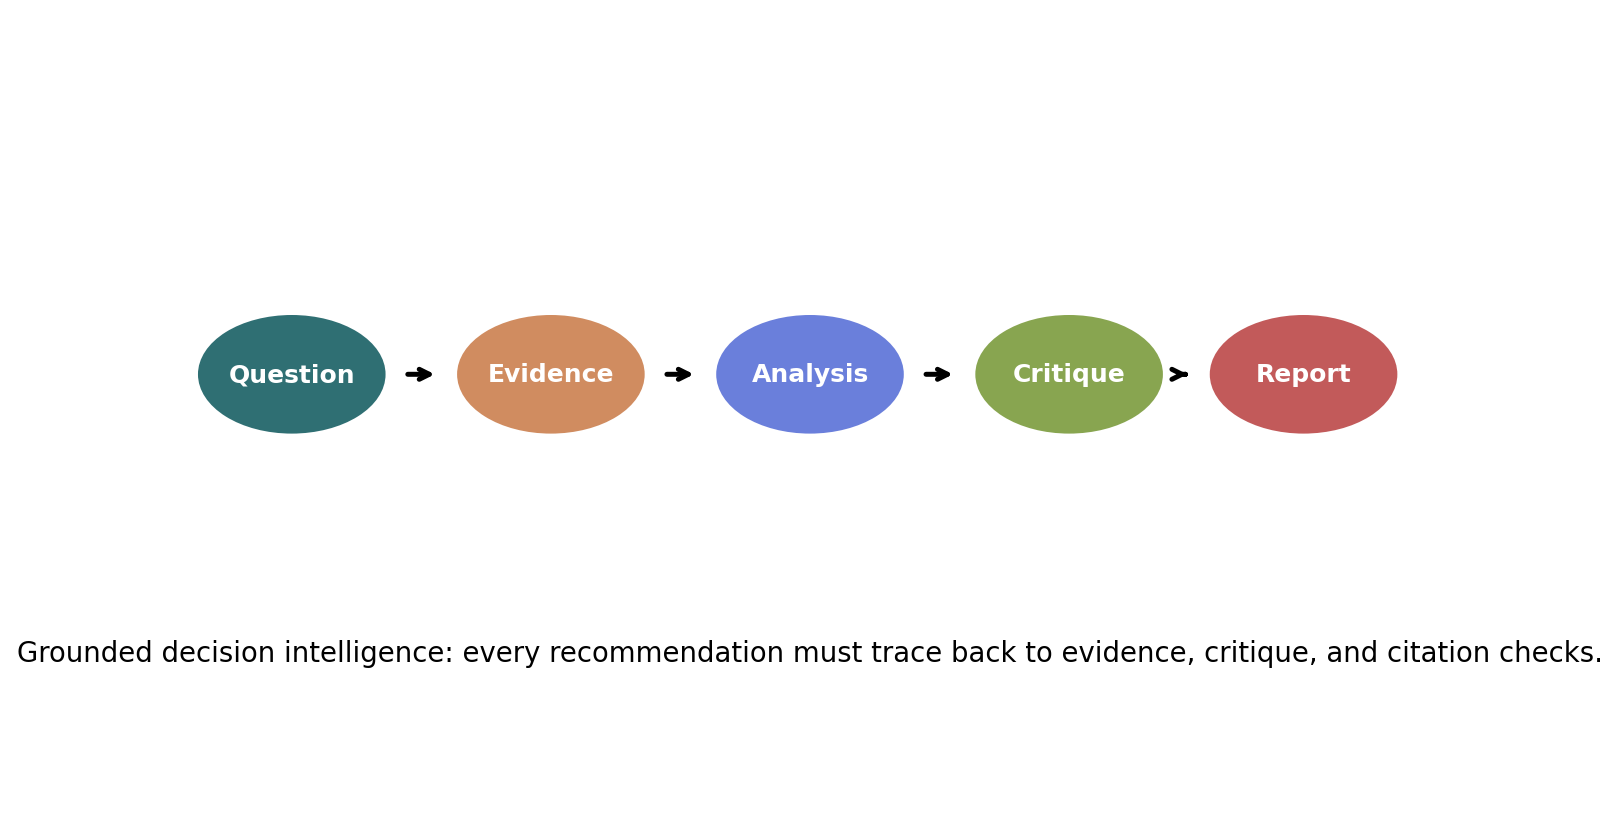
\includegraphics[width=0.96\linewidth,height=0.78\textheight,keepaspectratio]{assets/conceptual_grounding_pipeline.png}
\caption{Conceptual grounding pipeline from user question to evidence-backed synthesis.}
\label{fig:conceptual-grounding}
\end{figure}
\FloatBarrier


\section{Agent Responsibilities}
Each agent owns one responsibility. Planner decomposes the task; Research retrieves sources; Analyst computes metrics and tables; Critic searches for weaknesses; Fact-Checker grounds claims; Visualization creates charts and diagrams; Report Writer produces Markdown, LaTeX, and PDF artifacts; Evaluator scores output quality; Presentation exports slides; Memory persists the run. The tables below are generated from workflow state and use adaptive column widths to avoid text overlap.


\begin{table}[!htbp]
\centering
\caption{Agent Roles}
\label{tab:state-table-1}
\begingroup
\scriptsize
\setlength{\tabcolsep}{2.8pt}
\renewcommand{\arraystretch}{1.35}
\begin{adjustbox}{max width=\textwidth}
\begin{tabularx}{\textwidth}{@{}>{\RaggedRight\arraybackslash}p{0.16\textwidth}YYY@{}}
\toprule
\textbf{Agent} & \textbf{Responsibility} & \textbf{Input} & \textbf{Output} \\
\midrule
Planner & Task decomposition and routing & User query & Execution plan (PlanStep list) \\
Research & Evidence retrieval & Query and plan & Ranked Source objects \\
Analyst & Metrics, comparisons, formulas & Retrieved sources & Analysis tables and metrics \\
Critic & Weakness and risk review & Analysis and sources & needs\_revision flag and critique \\
Fact-Checker & Claim grounding & Approved analysis & ClaimCheck objects with citations \\
Visualization & Figures and diagrams & Workflow state snapshot & PNG, SVG, and Mermaid assets \\
Report Writer & Academic synthesis & Full workflow state & Markdown, LaTeX, and PDF reports \\
Evaluator & Rubric scoring & Report and figures & EvaluationScore JSON/Markdown \\
Presentation & Stakeholder communication & Evaluated state & Markdown and PPTX slides \\
Memory & Persistence & Completed workflow state & SQLite run record \\
\bottomrule
\end{tabularx}
\end{adjustbox}
\endgroup
\end{table}
\FloatBarrier


\begin{table}[!htbp]
\centering
\caption{Framework Comparison}
\label{tab:state-table-2}
\begingroup
\scriptsize
\setlength{\tabcolsep}{2.8pt}
\renewcommand{\arraystretch}{1.35}
\begin{adjustbox}{max width=\textwidth}
\begin{tabularx}{\textwidth}{@{}>{\RaggedRight\arraybackslash}p{0.16\textwidth}YYY@{}}
\toprule
\textbf{Framework} & \textbf{Strengths} & \textbf{Limitations} & \textbf{Suitability for This Project} \\
\midrule
LangGraph & Typed graph orchestration with conditional edges & Requires explicit state design & Best fit: mirrors critique and evaluation loops \\
Google ADK & Code-first agent toolkit with Google ecosystem deployment & Younger ecosystem and vendor coupling & Useful for Gemini/Vertex deployments, not required here \\
AutoGen & Conversational multi-agent patterns & Can become chat-loop centric & Good for research prototypes; less explicit graph control \\
CrewAI & Role/task abstraction is easy to teach & Less explicit low-level routing & Suitable for sequential crews, not revision gates \\
Semantic Kernel & Enterprise-friendly plugins and planners & Broad SDK surface area & Strong for Microsoft stacks; heavier than needed \\
\bottomrule
\end{tabularx}
\end{adjustbox}
\endgroup
\end{table}
\FloatBarrier


\begin{table}[!htbp]
\centering
\caption{API Endpoints}
\label{tab:state-table-3}
\begingroup
\footnotesize
\setlength{\tabcolsep}{2.8pt}
\renewcommand{\arraystretch}{1.35}
\begin{adjustbox}{max width=\textwidth}
\begin{tabularx}{\textwidth}{@{}>{\RaggedRight\arraybackslash}p{0.31\textwidth}>{\RaggedRight\arraybackslash}p{0.10\textwidth}Y@{}}
\toprule
\textbf{Endpoint} & \textbf{Method} & \textbf{Purpose} \\
\midrule
/health & GET & Service readiness check \\
/run & POST & Execute the full agentic workflow \\
/runs/\{run\_id\} & GET & Retrieve stored run metadata and serialized state \\
/runs/\{run\_id\}/report & GET & Download the generated Markdown report \\
/runs/\{run\_id\}/presentation & GET & Download the presentation artifact \\
/runs/\{run\_id\}/figures & GET & List paths to generated figure files \\
\bottomrule
\end{tabularx}
\end{adjustbox}
\endgroup
\end{table}
\FloatBarrier


\begin{table}[!htbp]
\centering
\caption{Evaluation Rubric}
\label{tab:state-table-4}
\begingroup
\footnotesize
\setlength{\tabcolsep}{2.8pt}
\renewcommand{\arraystretch}{1.35}
\begin{adjustbox}{max width=\textwidth}
\begin{tabularx}{\textwidth}{@{}>{\RaggedRight\arraybackslash}p{0.18\textwidth}Y>{\RaggedRight\arraybackslash}p{0.10\textwidth}@{}}
\toprule
\textbf{Criterion} & \textbf{Description} & \textbf{Weight} \\
\midrule
Factuality & Share of claims supported by retrieved sources & 15\% \\
Relevance & Alignment between query, plan, and final report & 12\% \\
Completeness & Presence of required sections, tables, figures, and formulas & 12\% \\
Structure & Logical organization and academic readability & 10\% \\
Citation quality & Traceable references and citation markers & 15\% \\
Clarity & Plain-language explanations of technical decisions & 10\% \\
Visual quality & Architecture diagrams, charts, and labeled figures & 13\% \\
Reproducibility & Mock mode, tests, scripts, Docker, and saved artifacts & 13\% \\
\bottomrule
\end{tabularx}
\end{adjustbox}
\endgroup
\end{table}
\FloatBarrier


\begin{table}[!htbp]
\centering
\caption{Limitations and Mitigations}
\label{tab:state-table-5}
\begingroup
\footnotesize
\setlength{\tabcolsep}{2.8pt}
\renewcommand{\arraystretch}{1.35}
\begin{adjustbox}{max width=\textwidth}
\begin{tabularx}{\textwidth}{@{}>{\RaggedRight\arraybackslash}p{0.22\textwidth}>{\RaggedRight\arraybackslash}p{0.25\textwidth}Y@{}}
\toprule
\textbf{Limitation} & \textbf{Impact} & \textbf{Mitigation} \\
\midrule
Static mock corpus & Evidence may be stale or incomplete & Deterministic grading; optional live search adapters \\
Real LLM dependency in production & Non-deterministic outputs without keys & USE\_MOCK\_LLM=true default; provider adapters behind tools \\
Citation verification limits & Tag-level checks miss entailment errors & Fact-checker gates claims; human review required \\
Clinical prototype scope & Not validated for patient-specific decisions & Explicit limitations, ethics section, no diagnosis claims \\
Human review requirement & Automation bias if outputs are trusted blindly & Critic mandates limitations; evaluator threshold gate \\
\bottomrule
\end{tabularx}
\end{adjustbox}
\endgroup
\end{table}
\FloatBarrier


\section{Workflow and State Model}
The workflow is stateful rather than conversationally implicit. \texttt{WorkflowState} contains the query, plan, sources, notes, analysis values, tables, critique, revision flags, claim checks, figure paths, report paths, evaluation scores, status, and errors. Conditional routing occurs after the Critic and Evaluator, which makes the graph agentic: weak evidence can route back to Research, and a low report score can route back to Report Writer before finalization.


\begin{table}[!htbp]
\centering
\caption{Conditional Routing Rules}
\label{tab:routing-rules}
\begingroup
\footnotesize
\setlength{\tabcolsep}{2.8pt}
\renewcommand{\arraystretch}{1.35}
\begin{adjustbox}{max width=\textwidth}
\begin{tabularx}{\textwidth}{@{}>{\RaggedRight\arraybackslash}p{0.18\textwidth}Y>{\RaggedRight\arraybackslash}p{0.24\textwidth}@{}}
\toprule
\textbf{Decision point} & \textbf{Condition} & \textbf{Next node} \\
\midrule
Critic & Evidence is insufficient and revision budget remains & Research Agent \\
Critic & Evidence is acceptable & Fact-Checker Agent \\
Evaluator & Quality score $Q < \tau$ where $\tau=78$ & Report Writer Agent \\
Evaluator & Quality score $Q \geq \tau$ & Presentation Agent \\
Presentation & Slide artifact generated & Memory Agent \\
\bottomrule
\end{tabularx}
\end{adjustbox}
\endgroup
\end{table}
\FloatBarrier


\section{Mathematical Formulation}
The Planner decomposes a user request $q$ into ordered tasks:
\begin{equation}
T(q)=\{t_1,t_2,\ldots,t_n\}, \qquad t_i=(d_i,a_i,D_i)
\end{equation}
where $d_i$ is the task description, $a_i$ is the assigned agent, and $D_i$ is the dependency set.

Mock retrieval ranks each source $x$ with a transparent heuristic:
\begin{equation}
S(x,q)=\lambda_1\,\operatorname{overlap}(x,q)+\lambda_2\,\operatorname{credibility}(x)+\lambda_3\,\operatorname{tag\_match}(x,q).
\end{equation}
This keeps grading deterministic while preserving a clear extension point for live search.

The confidence score is modeled as a weighted evidence aggregate:
\begin{equation}
C = 100 \cdot \frac{\sum_{i=1}^n w_i s_i}{\sum_{i=1}^n w_i},
\end{equation}
where $s_i$ is a source-quality or coverage signal and $w_i$ is its weight. In this run, $C=95.5/100$.

The evaluator combines quality dimensions into an overall score:
\begin{equation}
Q=\frac{F+R+M+S+K+L+V+P}{8},
\end{equation}
where $F$ is factuality, $R$ relevance, $M$ completeness, $S$ structure, $K$ citation quality, $L$ clarity, $V$ visual quality, and $P$ reproducibility.

The revision gate is:
\begin{equation}
r=\begin{cases}
1, & Q < \tau \ \text{and revision budget remains},\\
0, & Q \geq \tau \ \text{or budget is exhausted},
\end{cases}
\qquad \tau=78.
\end{equation}
When $r=1$, the graph returns to a previous generation stage instead of silently accepting a weak artifact.

\section{Algorithmic Workflow}
\begin{lstlisting}[caption={Algorithm 1: Conditional multi-agent execution},label={lst:agentic-algorithm}]
Input: query q, threshold tau, maximum revisions m
state <- initialize WorkflowState(q)
state.plan <- Planner(q)
state.sources <- Research(state.plan)
state.analysis <- Analyst(state.sources)
state.critique <- Critic(state.analysis, state.sources)
while state.needs_revision and state.revision_count < m:
    state.revision_count <- state.revision_count + 1
    state.sources <- Research(state.critique)
    state.analysis <- Analyst(state.sources)
    state.critique <- Critic(state.analysis, state.sources)
state.claim_checks <- FactChecker(state.sources, state.analysis)
state.figures <- Visualization(state)
state.report <- ReportWriter(state)
state.evaluation <- Evaluator(state.report, state.figures)
while state.evaluation.total < tau and state.revision_count < m:
    state.revision_count <- state.revision_count + 1
    state.report <- ReportWriter(state)
    state.evaluation <- Evaluator(state.report, state.figures)
state.report <- ReportWriter(state)  # final pass with final score
state.presentation <- Presentation(state.report)
Memory.save(state)
return state
\end{lstlisting}

\begin{lstlisting}[caption={Algorithm 2: Claim grounding and citation gating},label={lst:claim-gating}]
Input: candidate claims, retrieved sources
for each claim in candidate claims:
    matching_sources <- sources with related tags, title terms, or summaries
    if matching_sources is empty:
        mark claim unsupported
        attach no generated citation
    else:
        mark claim supported
        attach only retrieved-source citation markers
return claim check list
\end{lstlisting}

\section{Evidence and Citation Strategy}
The retrieval component ranks sources by query overlap, credibility, and tags. The fact checker only cites already-retrieved sources and does not invent references. The strongest evidence themes in this run were: evaluation (9), clinical (8), agentic (8), ethics (6), framework (5), risk (4), decision\_support (3), reporting (3). Table~\ref{tab:evidence-sources} samples the evidence base used by the generated report.


\begin{table}[!htbp]
\centering
\caption{Representative Retrieved Evidence Sources}
\label{tab:evidence-sources}
\begingroup
\scriptsize
\setlength{\tabcolsep}{2.8pt}
\renewcommand{\arraystretch}{1.35}
\begin{adjustbox}{max width=\textwidth}
\begin{tabularx}{\textwidth}{@{}>{\RaggedRight\arraybackslash}p{0.13\textwidth}>{\RaggedRight\arraybackslash}p{0.08\textwidth}>{\RaggedRight\arraybackslash}p{0.11\textwidth}>{\RaggedRight\arraybackslash}p{0.20\textwidth}Y@{}}
\toprule
\textbf{Type} & \textbf{Year} & \textbf{Credibility} & \textbf{Tags} & \textbf{Title} \\
\midrule
paper & 2020 & 0.96 & clinical, decision\_support, risk, ethics & An Overview of Clinical Decision Support Systems: Benefits, Risks, and Strategies for Success \\
paper & 2005 & 0.94 & clinical, decision\_support, evaluation & Effects of Computerized Clinical Decision Support Systems on Practitioner Performance and Patient Outcomes \\
paper & 2005 & 0.94 & clinical, decision\_support, evaluation & Improving Clinical Practice Using Clinical Decision Support Systems: A Systematic Review of Trials \\
guideline & 2022 & 0.96 & clinical, ethics, reporting, evaluation & DECIDE-AI: New Reporting Guidelines to Bridge the Development-to-Implementation Gap in Clinical Artificial Intelligence \\
docs & 2026 & 0.84 & agentic, framework, adk & Agent Development Kit Multi-Agent Systems Documentation \\
policy & 2021 & 0.98 & clinical, ethics, governance, risk & Ethics and Governance of Artificial Intelligence for Health \\
guideline & 2020 & 0.97 & clinical, ethics, evaluation, reporting & CONSORT-AI Extension: Reporting Guidelines for Clinical Trials of Artificial Intelligence Interventions \\
guideline & 2020 & 0.97 & clinical, ethics, reporting & SPIRIT-AI Extension: Protocol Guidelines for Clinical Trials of Artificial Intelligence Interventions \\
paper & 2023 & 0.95 & clinical, medical, evaluation, llm & Large Language Models Encode Clinical Knowledge \\
paper & 2023 & 0.91 & hallucination, evaluation, risk & Survey of Hallucination in Natural Language Generation \\
paper & 2023 & 0.84 & agentic, multi\_agent, framework & AutoGen: Enabling Next-Gen LLM Applications via Multi-Agent Conversation \\
paper & 2020 & 0.94 & rag, retrieval, hallucination, evidence & Retrieval-Augmented Generation for Knowledge-Intensive NLP Tasks \\
\bottomrule
\end{tabularx}
\end{adjustbox}
\endgroup
\end{table}
\FloatBarrier


\section{Implementation Details}
The repository separates concerns into \texttt{app/agents}, \texttt{app/graph}, \texttt{app/tools}, \texttt{app/models}, \texttt{app/storage}, \texttt{app/ui}, and \texttt{scripts}. The graph runner uses LangGraph when available and a deterministic fallback runner otherwise. Tools handle retrieval, citation formatting, visualization, report generation, presentation export, and filesystem writes. This separation keeps the agents simple and makes the project easier to test.

\section{API, Storage, and Artifacts}
FastAPI provides health, run, report, presentation, and figure endpoints. SQLite stores run metadata and serialized state for later inspection. Generated artifacts are written to \texttt{outputs/} for run-specific files and \texttt{report/} for canonical submission files. The canonical report paths are \texttt{report/final\_report.tex}, \texttt{report/final\_report.pdf}, \texttt{report/final\_report.md}, and \texttt{report/references.bib}.

\section{User Interface and Panel Screenshots}
The Streamlit panel exposes the project without requiring graders to read code first. It includes topic input, mock/real mode selection, run execution, workflow inspection, agent outputs, evaluation metrics, figure previews, and download controls. Screenshot capture type: \texttt{browser}. Metadata: Captured current Streamlit UI viewport with Playwright/Chromium on port 8511 after seeded mock demo.


\begin{figure}[!htbp]
\centering
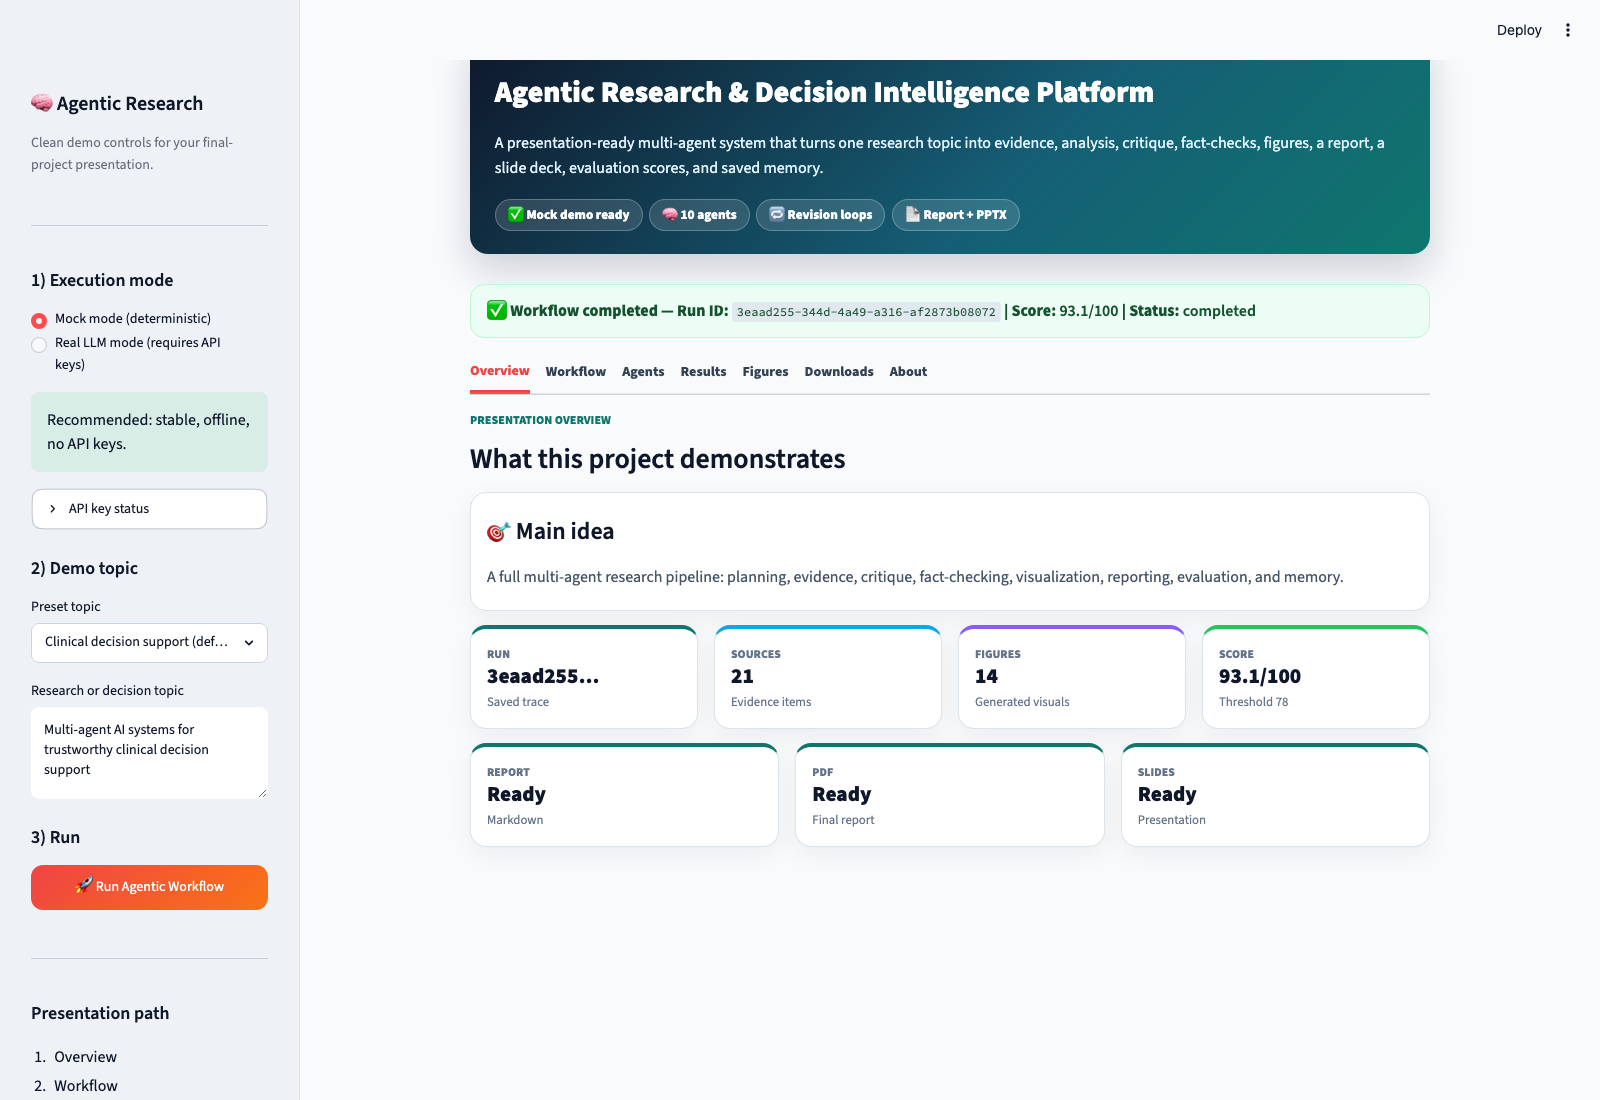
\includegraphics[width=0.98\linewidth,height=0.78\textheight,keepaspectratio]{assets/ui/ui_home.png}
\caption{Actual Streamlit Overview tab captured in a headless browser after mock demo run.}
\label{fig:ui-home}
\end{figure}
\FloatBarrier


\begin{figure}[!htbp]
\centering
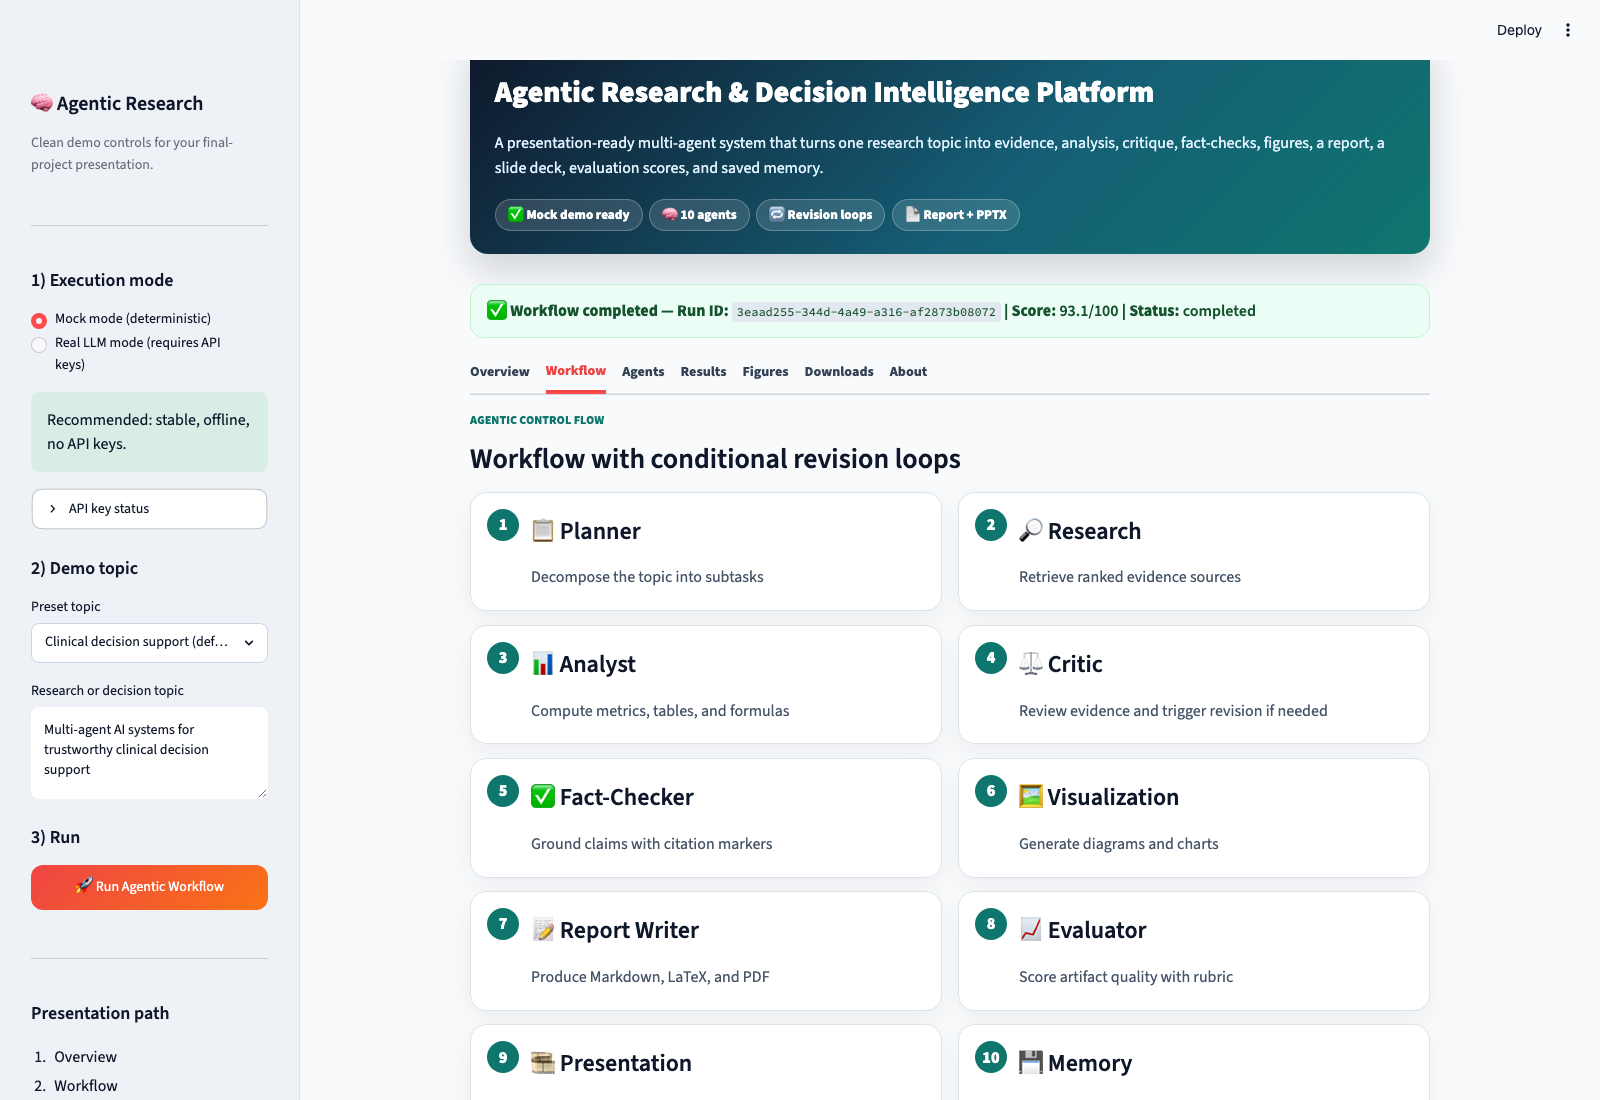
\includegraphics[width=0.98\linewidth,height=0.78\textheight,keepaspectratio]{assets/ui/ui_workflow.png}
\caption{Actual Streamlit Workflow tab captured in a headless browser after mock demo run.}
\label{fig:ui-workflow}
\end{figure}
\FloatBarrier


\begin{figure}[!htbp]
\centering
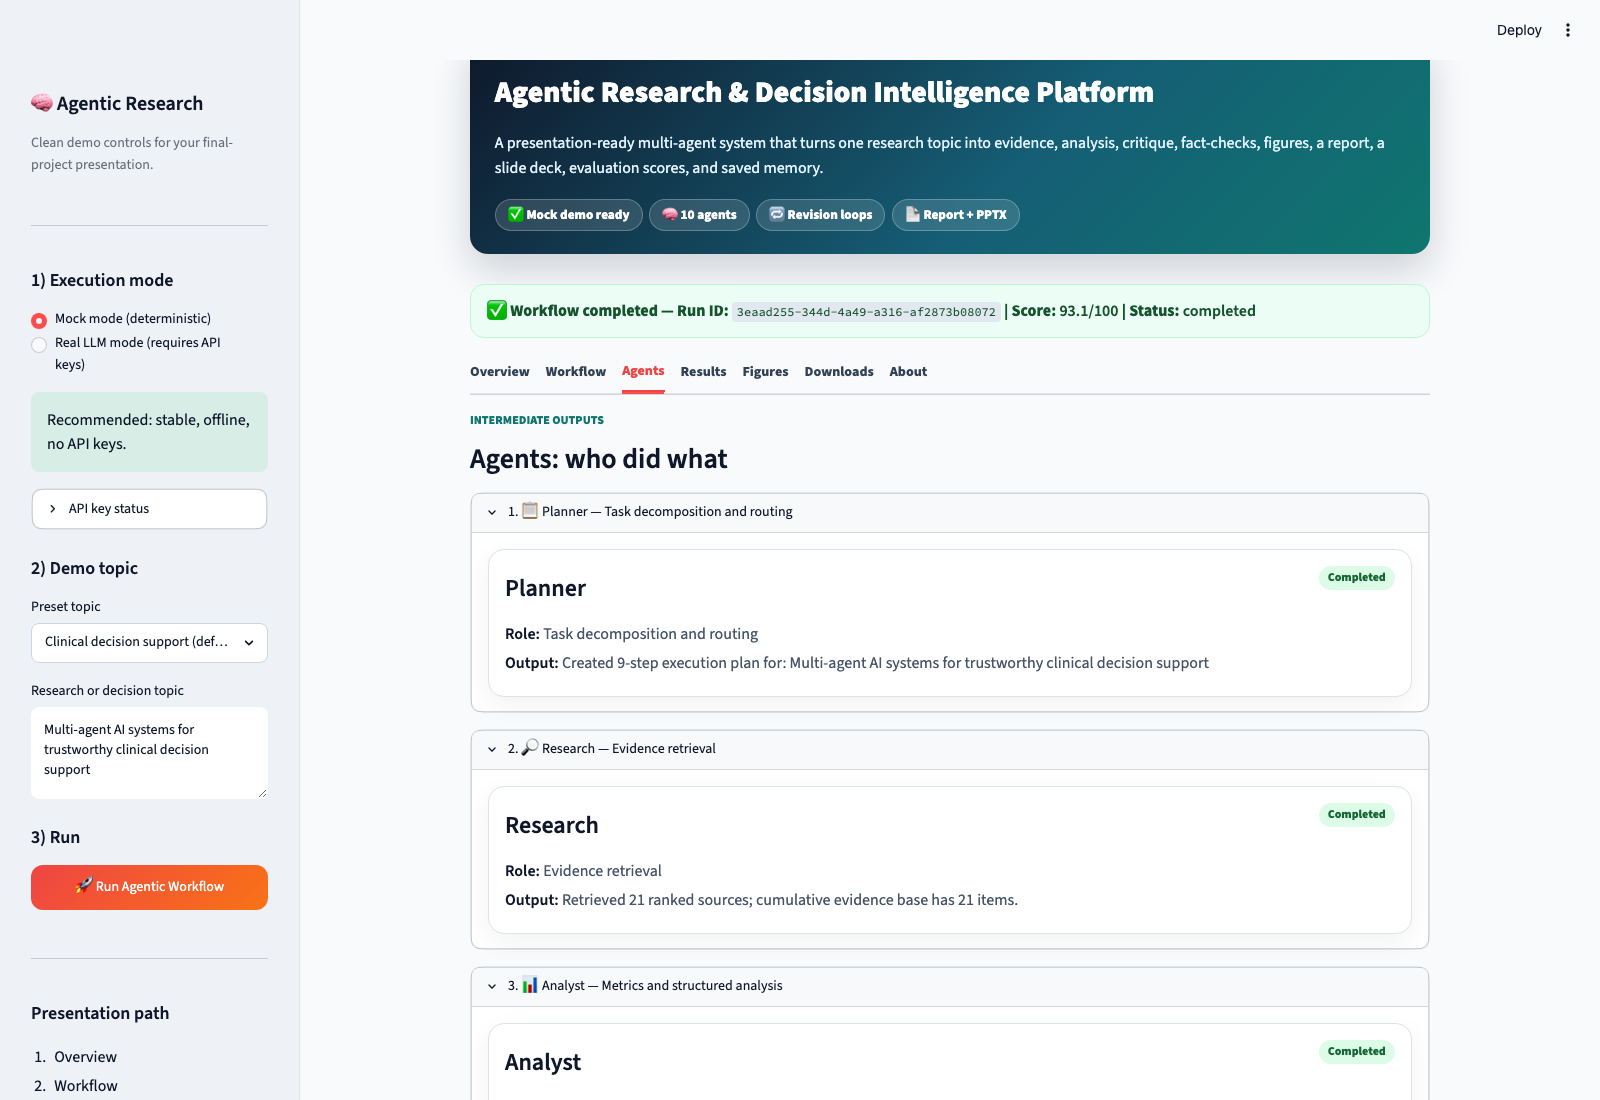
\includegraphics[width=0.98\linewidth,height=0.78\textheight,keepaspectratio]{assets/ui/ui_agent_outputs.png}
\caption{Actual Streamlit Agents tab captured in a headless browser after mock demo run.}
\label{fig:ui-agent-outputs}
\end{figure}
\FloatBarrier


\begin{figure}[!htbp]
\centering
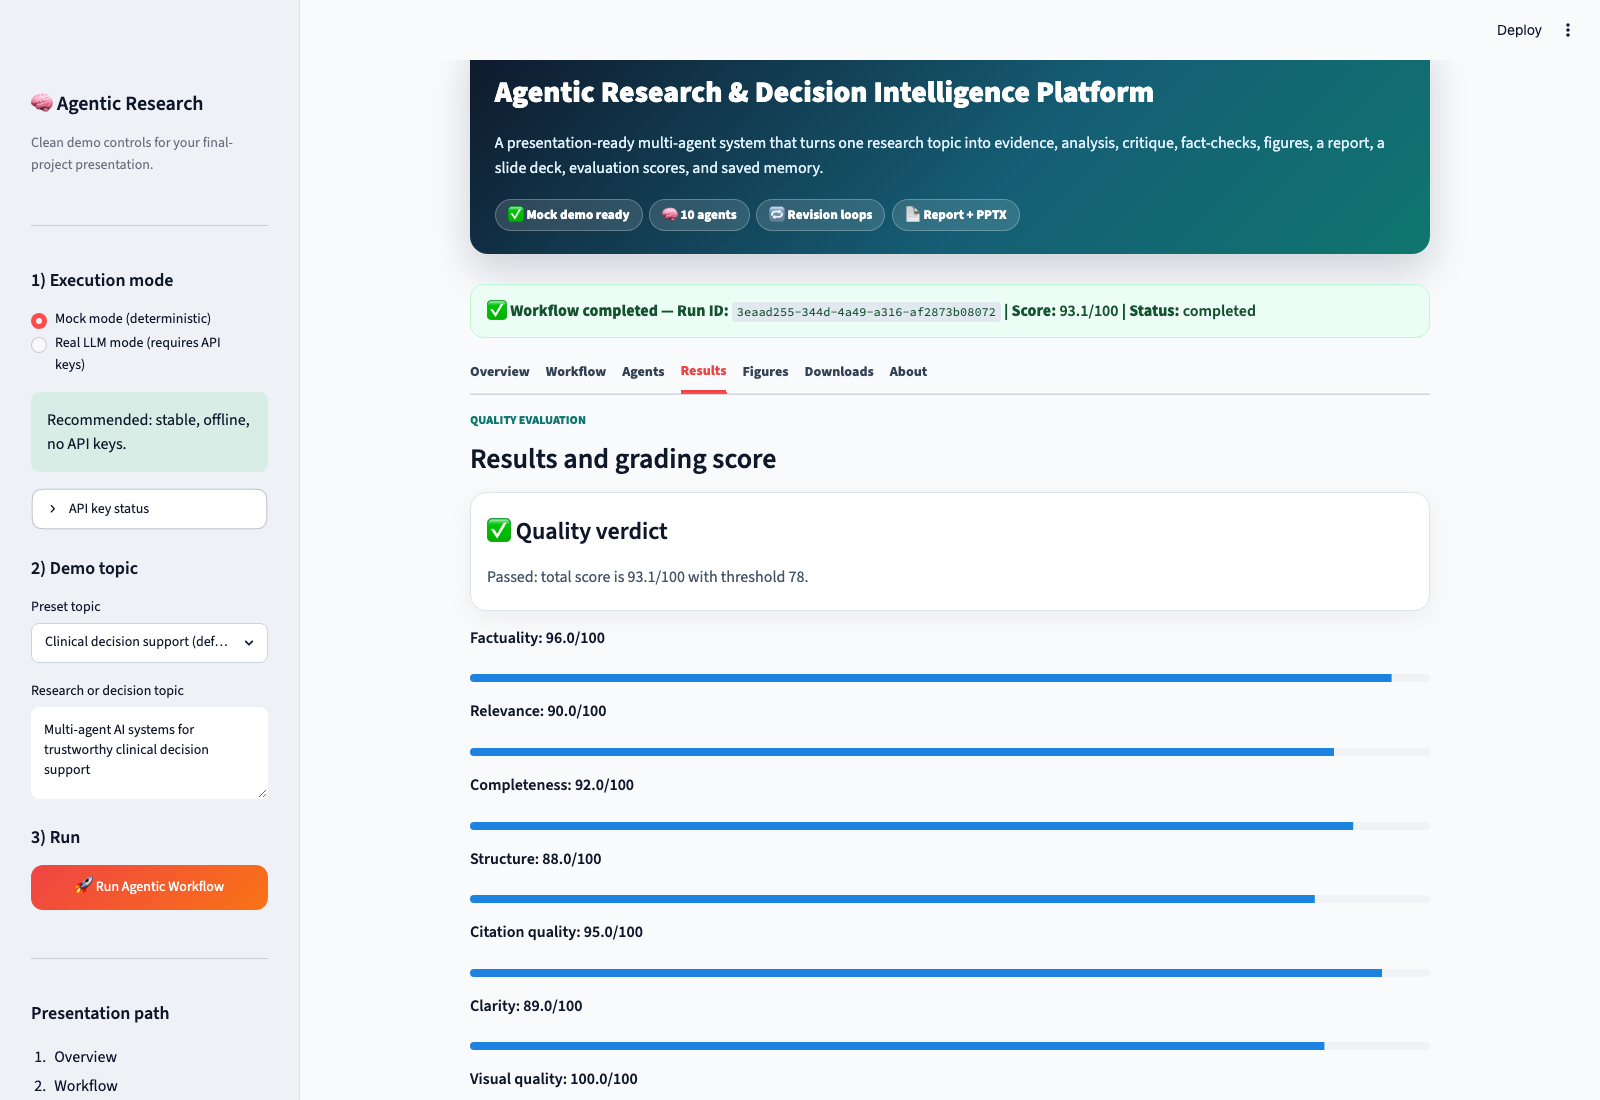
\includegraphics[width=0.98\linewidth,height=0.78\textheight,keepaspectratio]{assets/ui/ui_results.png}
\caption{Actual Streamlit Results tab captured in a headless browser after mock demo run.}
\label{fig:ui-results}
\end{figure}
\FloatBarrier


\begin{figure}[!htbp]
\centering
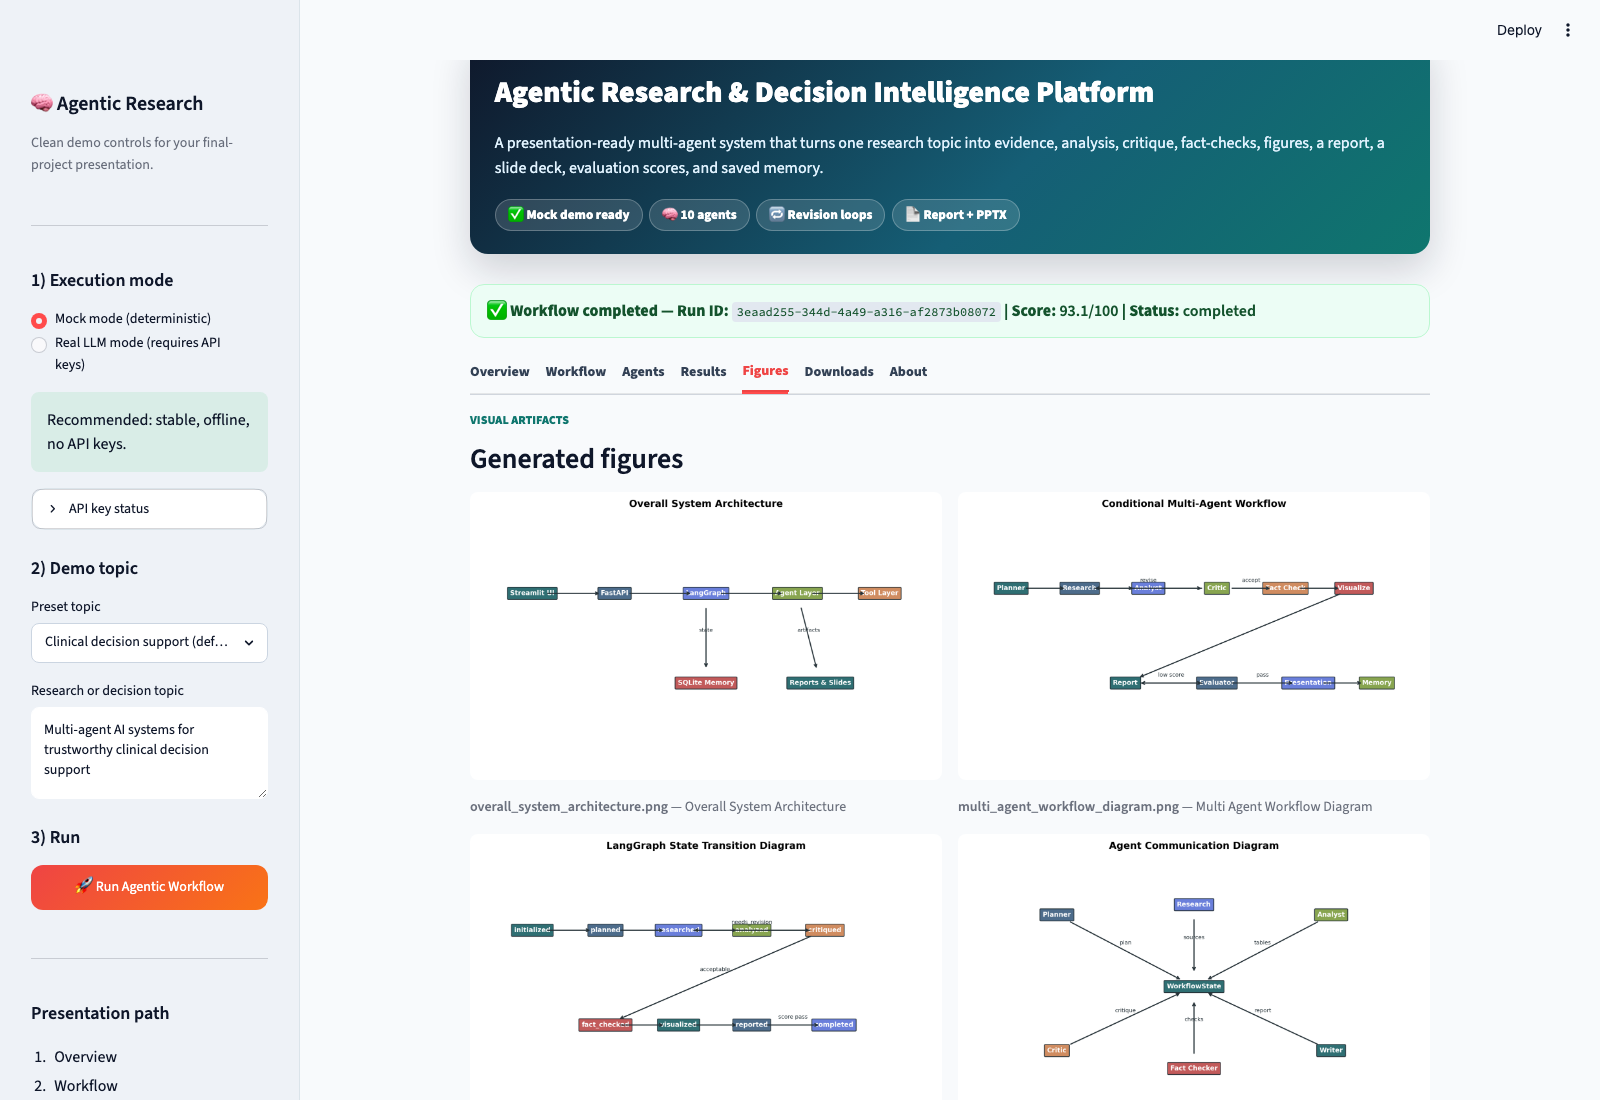
\includegraphics[width=0.98\linewidth,height=0.78\textheight,keepaspectratio]{assets/ui/ui_figures.png}
\caption{Actual Streamlit Figures tab captured in a headless browser after mock demo run.}
\label{fig:ui-figures}
\end{figure}
\FloatBarrier


\begin{figure}[!htbp]
\centering
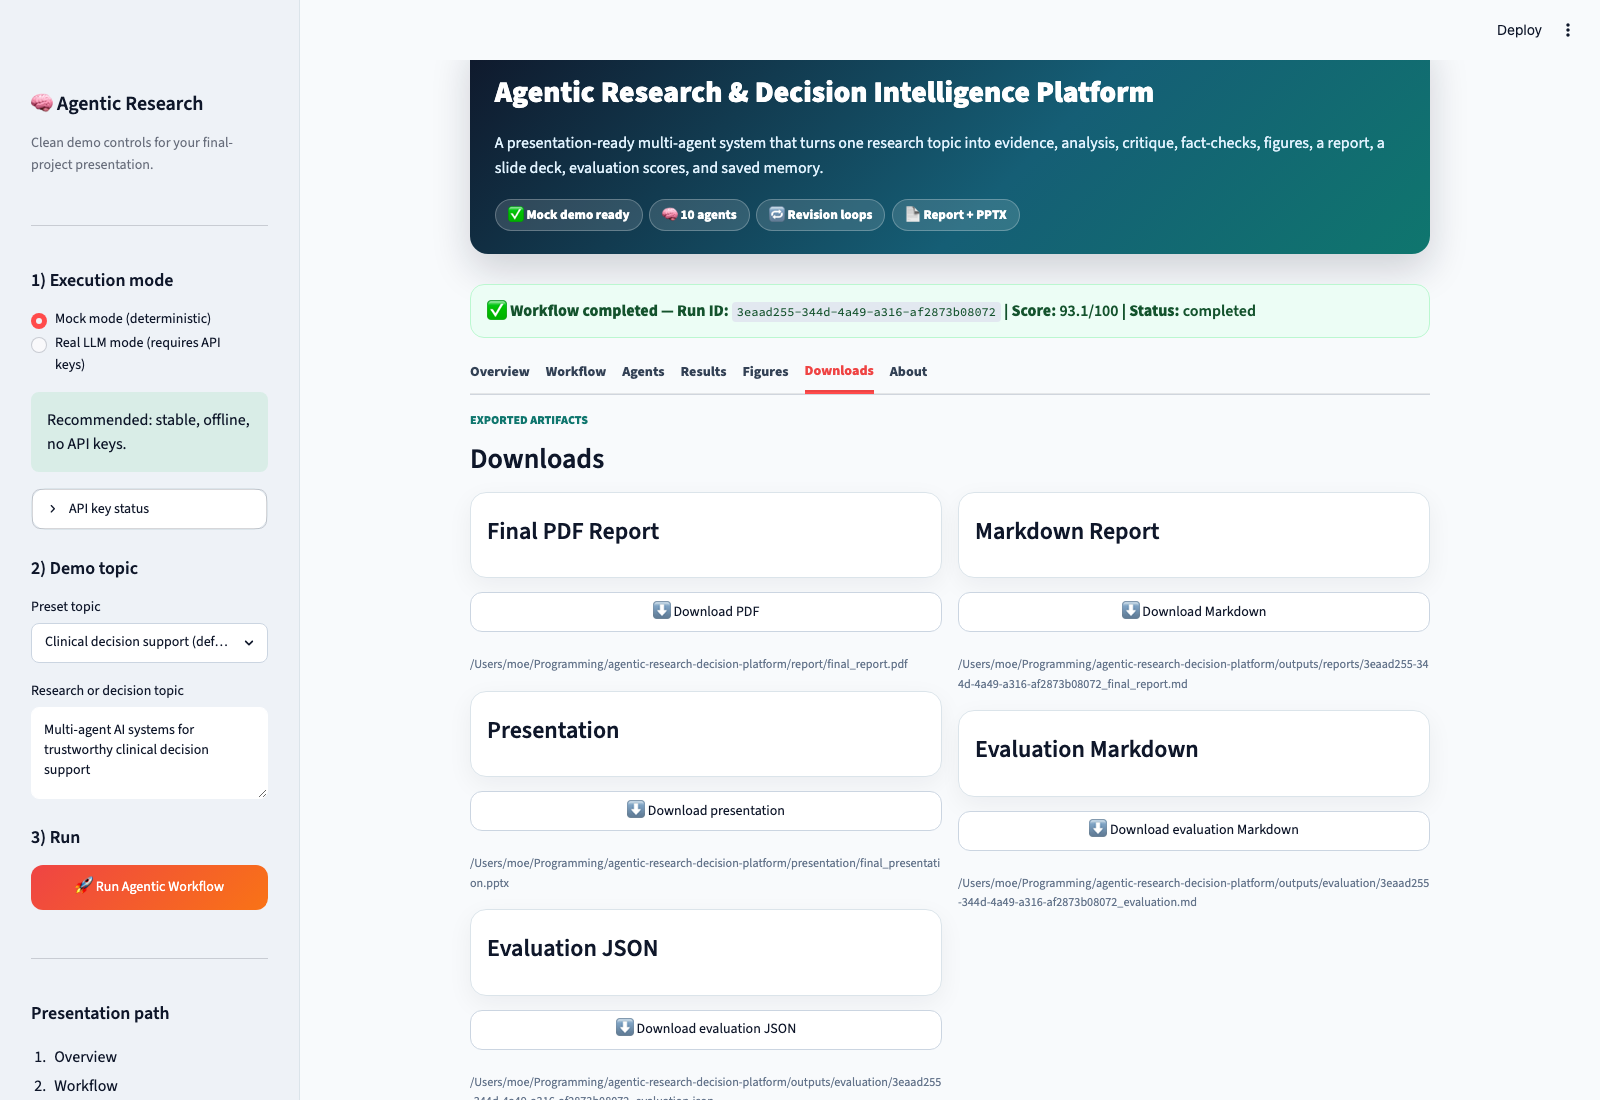
\includegraphics[width=0.98\linewidth,height=0.78\textheight,keepaspectratio]{assets/ui/ui_downloads.png}
\caption{Actual Streamlit Downloads tab captured in a headless browser after mock demo run.}
\label{fig:ui-downloads}
\end{figure}
\FloatBarrier


\begin{figure}[!htbp]
\centering
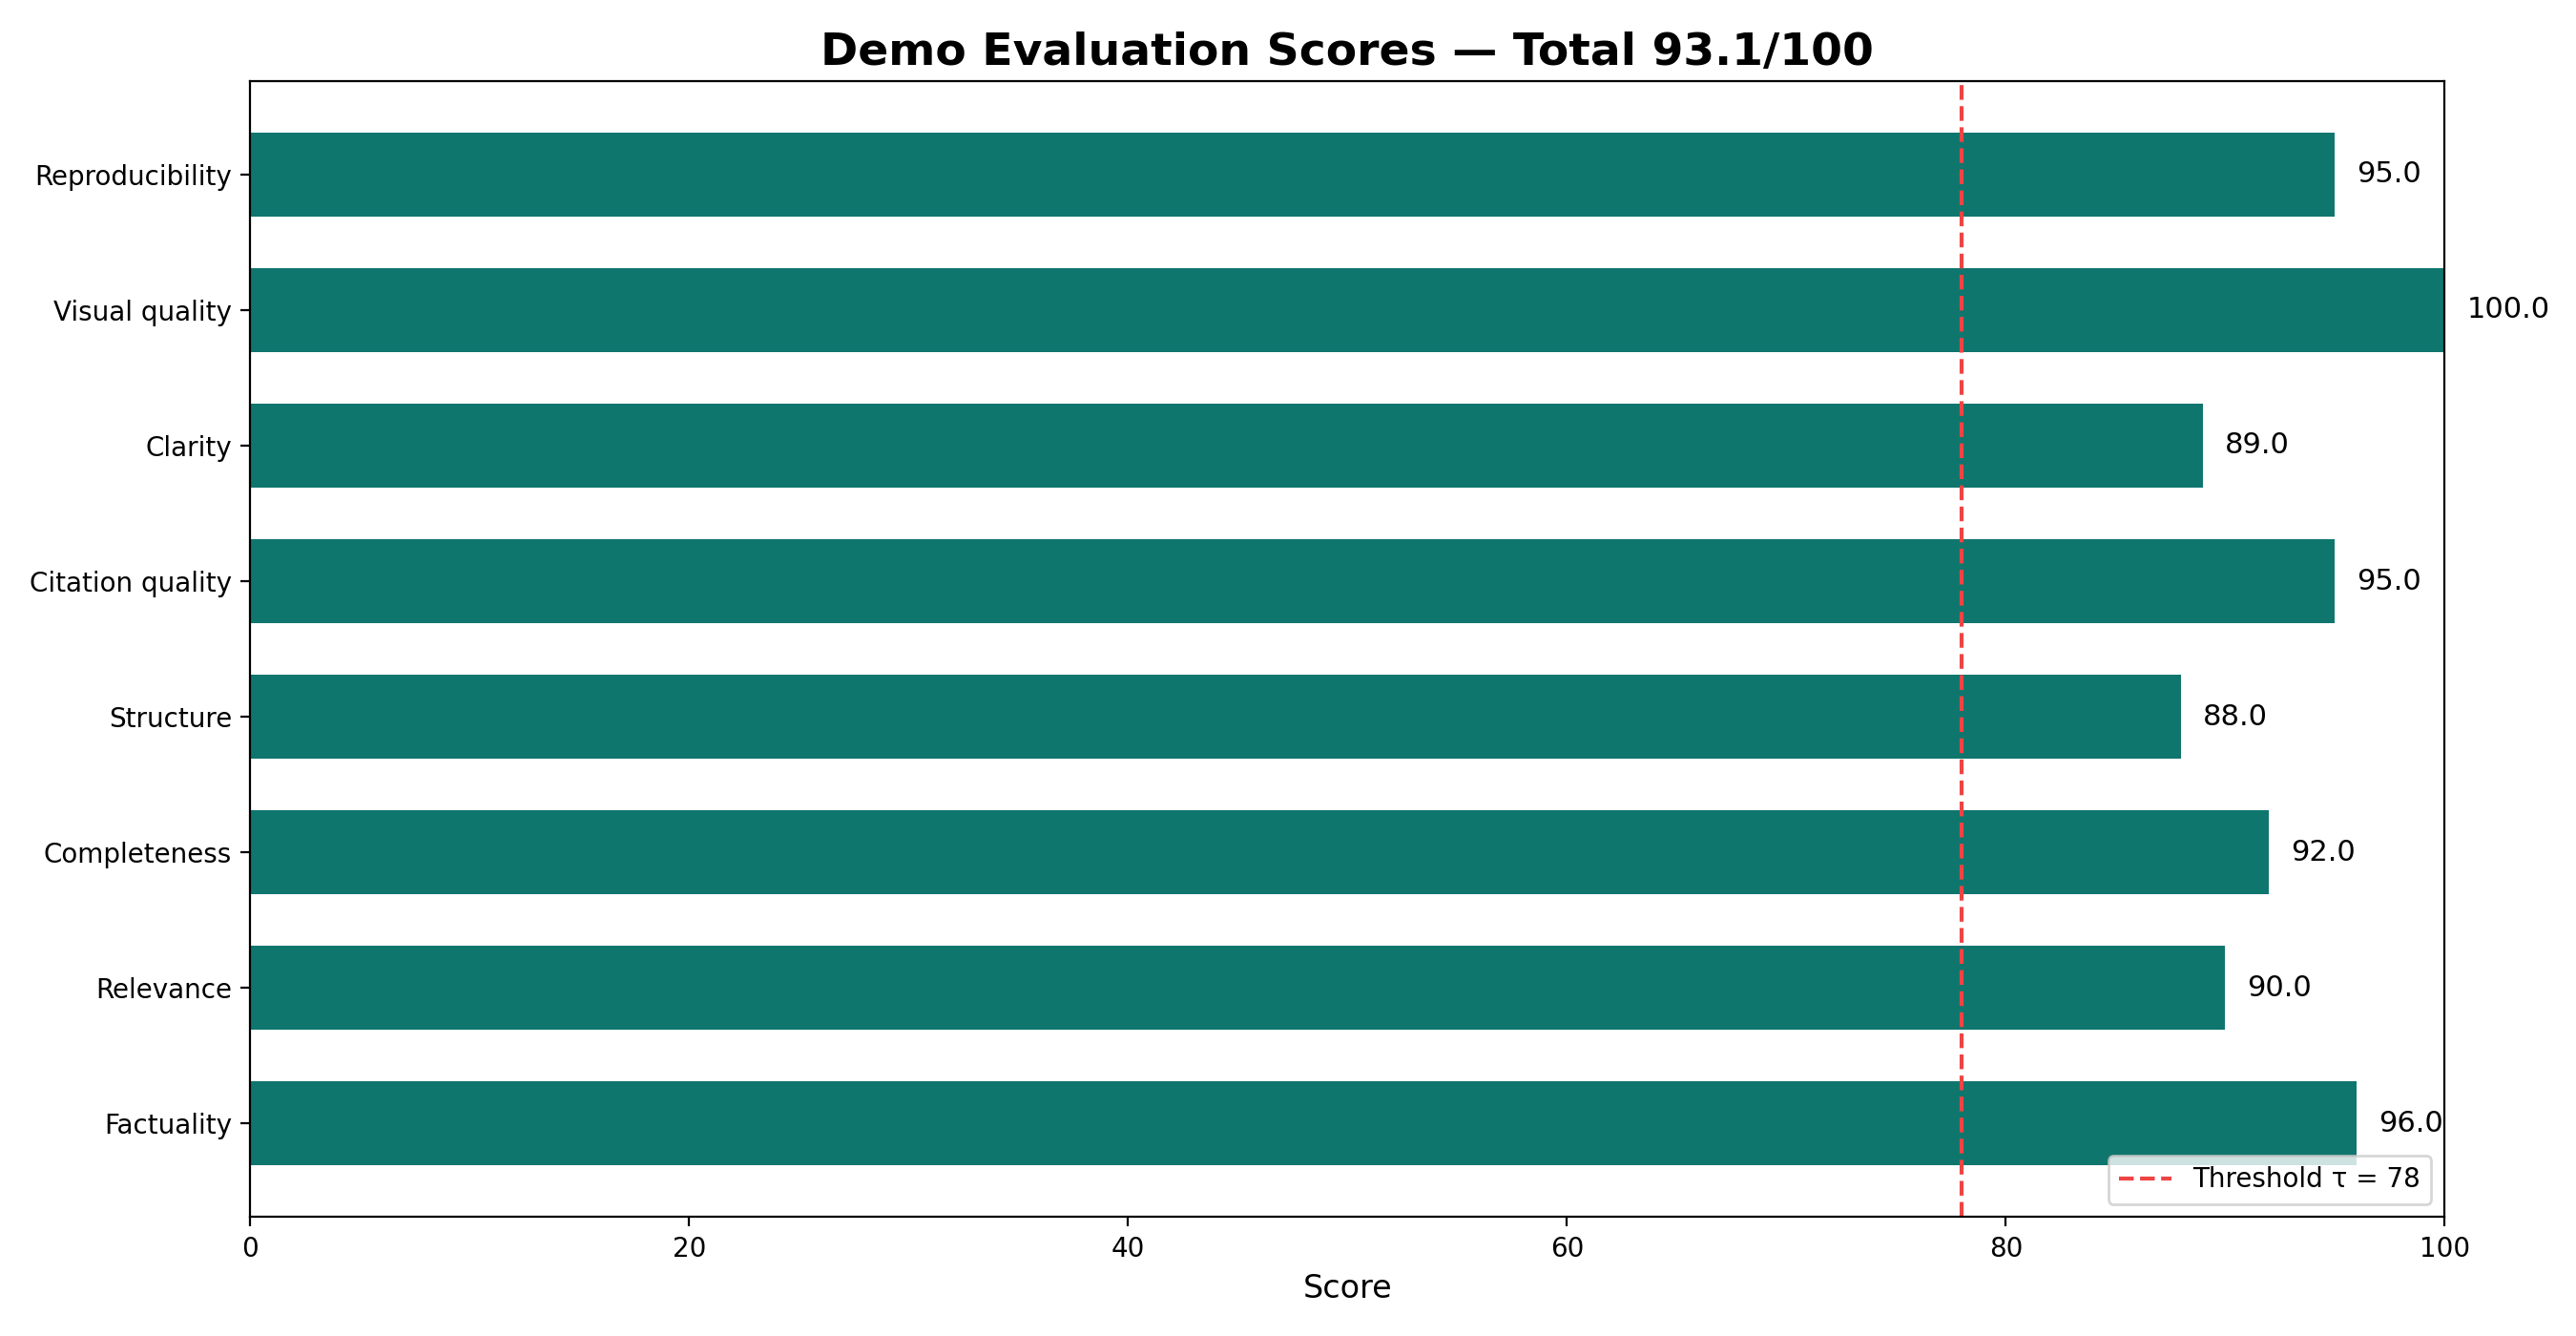
\includegraphics[width=0.95\linewidth,height=0.78\textheight,keepaspectratio]{assets/results/demo_evaluation_score.png}
\caption{Demo evaluation score panel generated from the reproducible workflow run.}
\label{fig:demo-eval}
\end{figure}
\FloatBarrier


\begin{figure}[!htbp]
\centering

\includegraphics[width=0.95\linewidth,height=0.78\textheight,keepaspectratio]{assets/results/demo_agent_workflow_result.png}
\caption{Demo workflow result panel summarizing run ID, status, sources, figures, and agent sequence.}
\label{fig:demo-workflow-result}
\end{figure}
\FloatBarrier


\begin{figure}[!htbp]
\centering
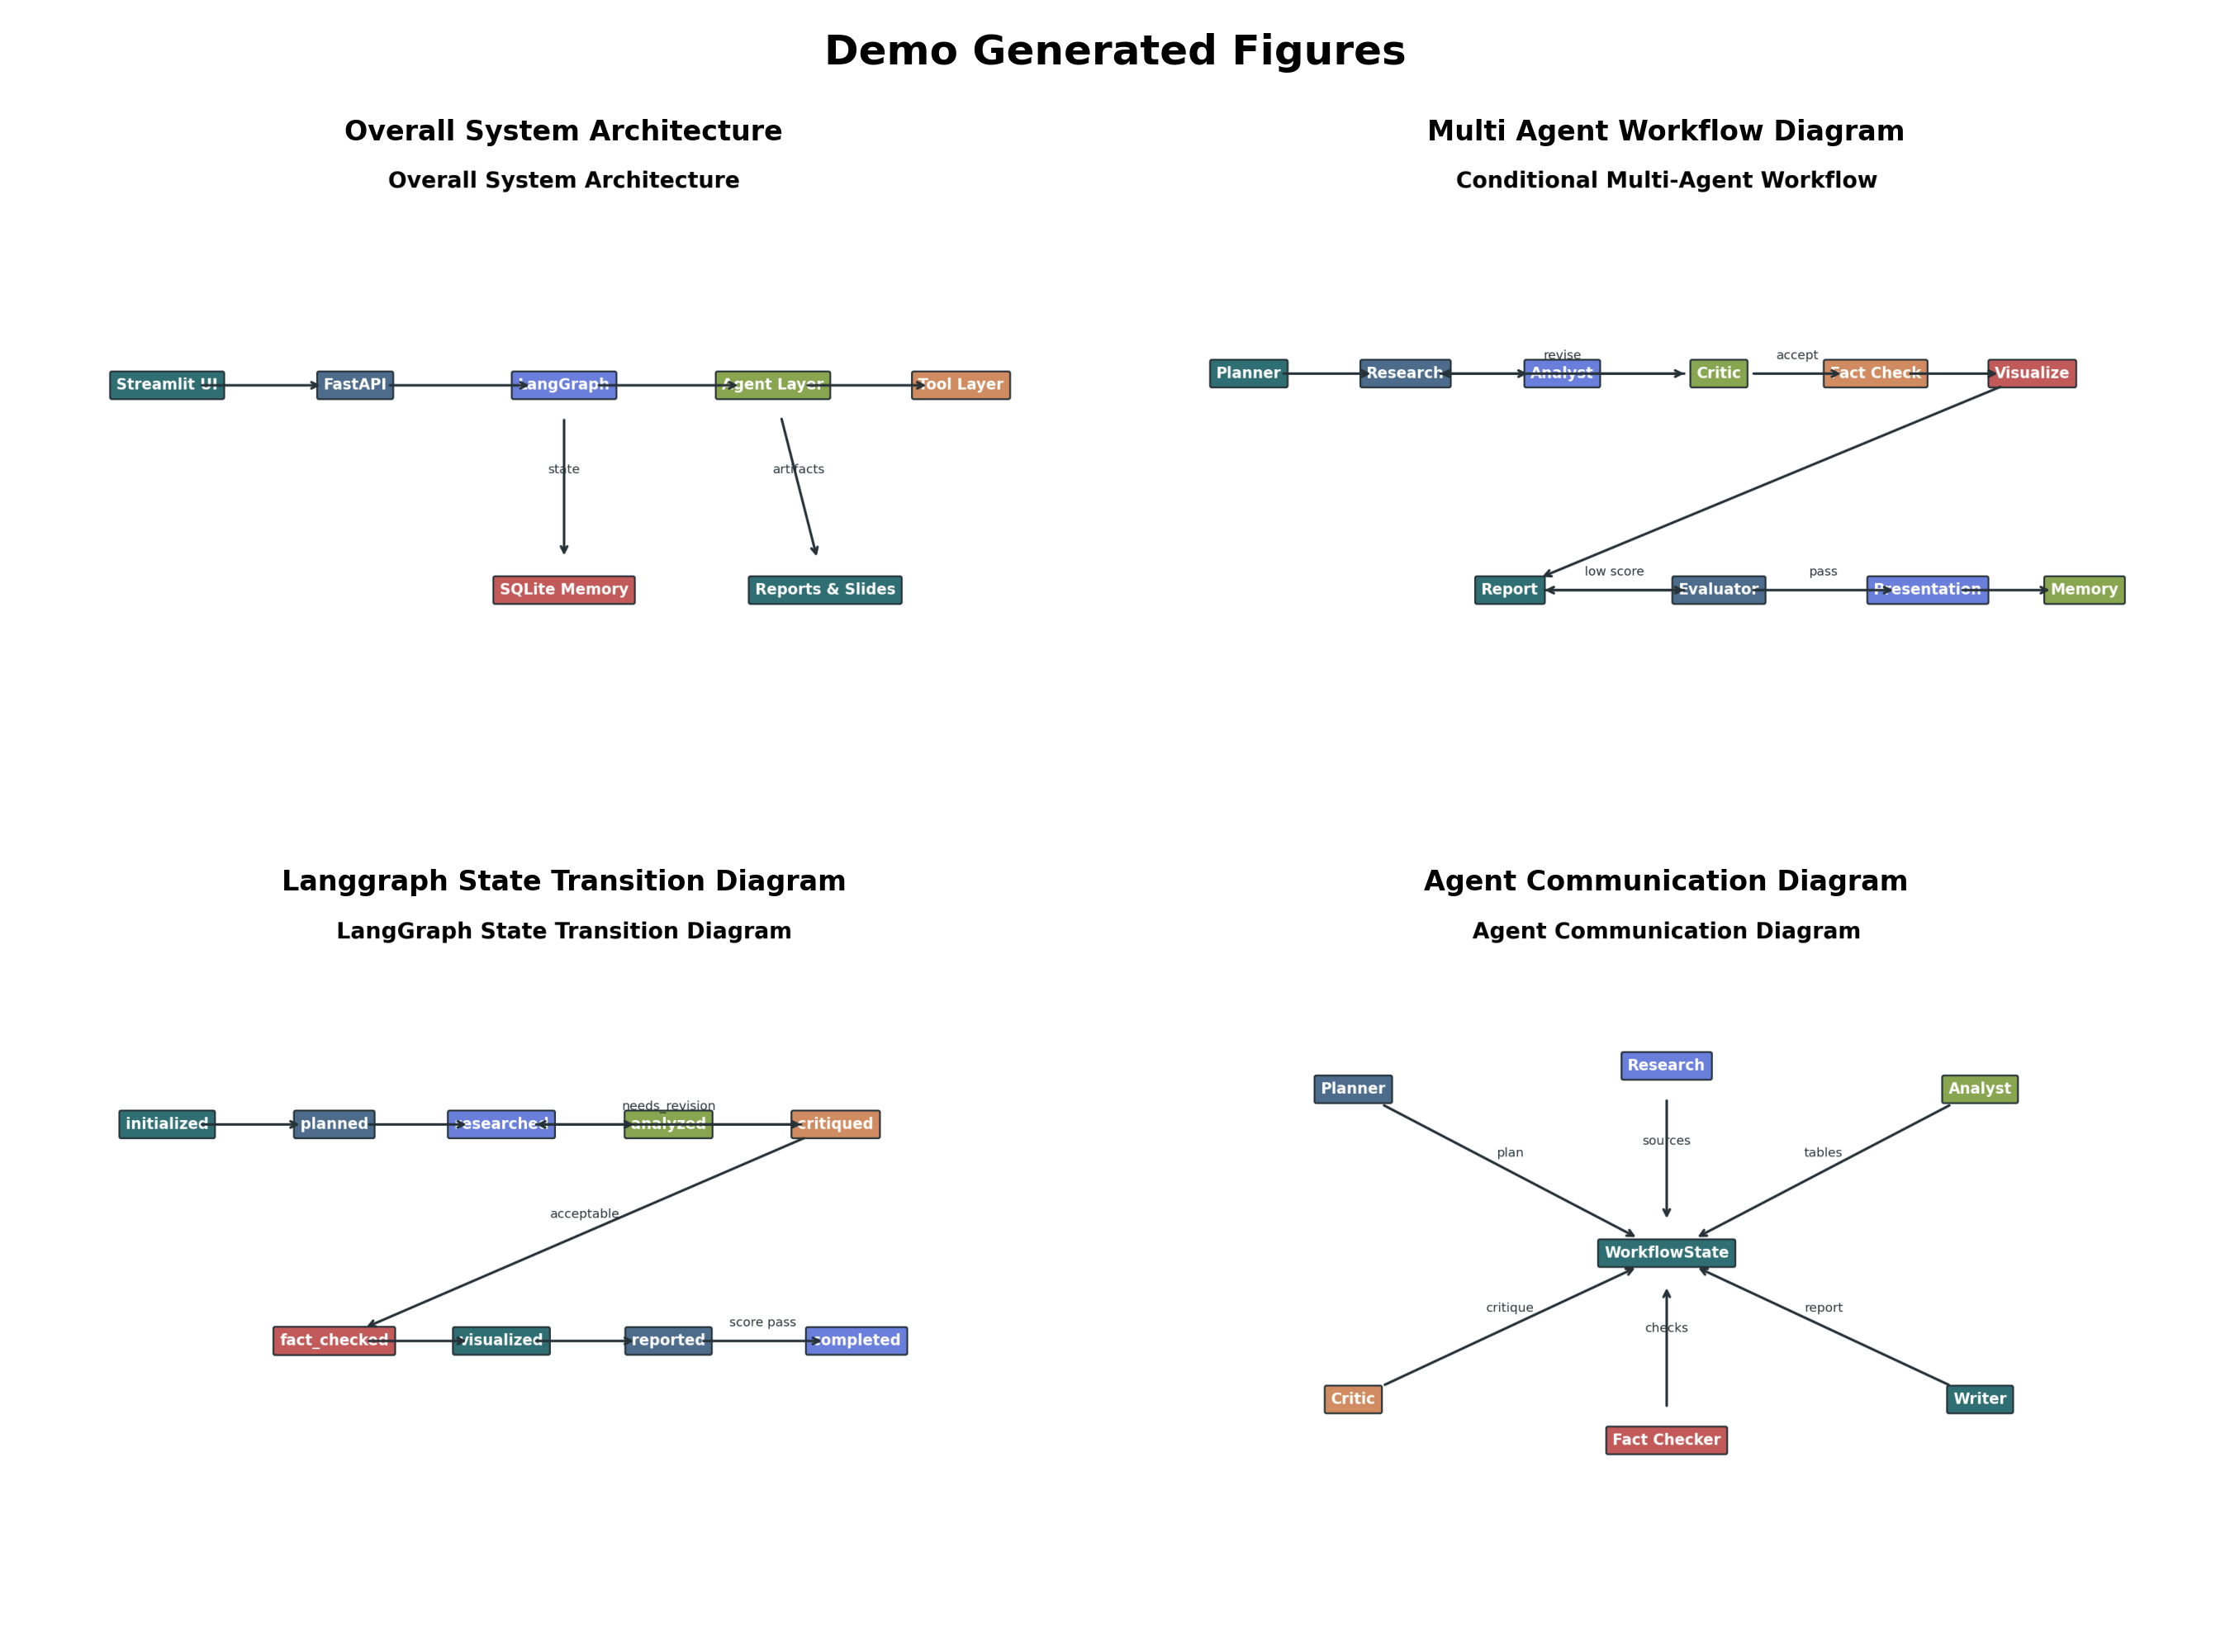
\includegraphics[width=0.95\linewidth,height=0.78\textheight,keepaspectratio]{assets/results/demo_generated_figures.png}
\caption{Demo gallery of generated figures used by the final report.}
\label{fig:demo-generated-figures}
\end{figure}
\FloatBarrier


\begin{figure}[!htbp]
\centering
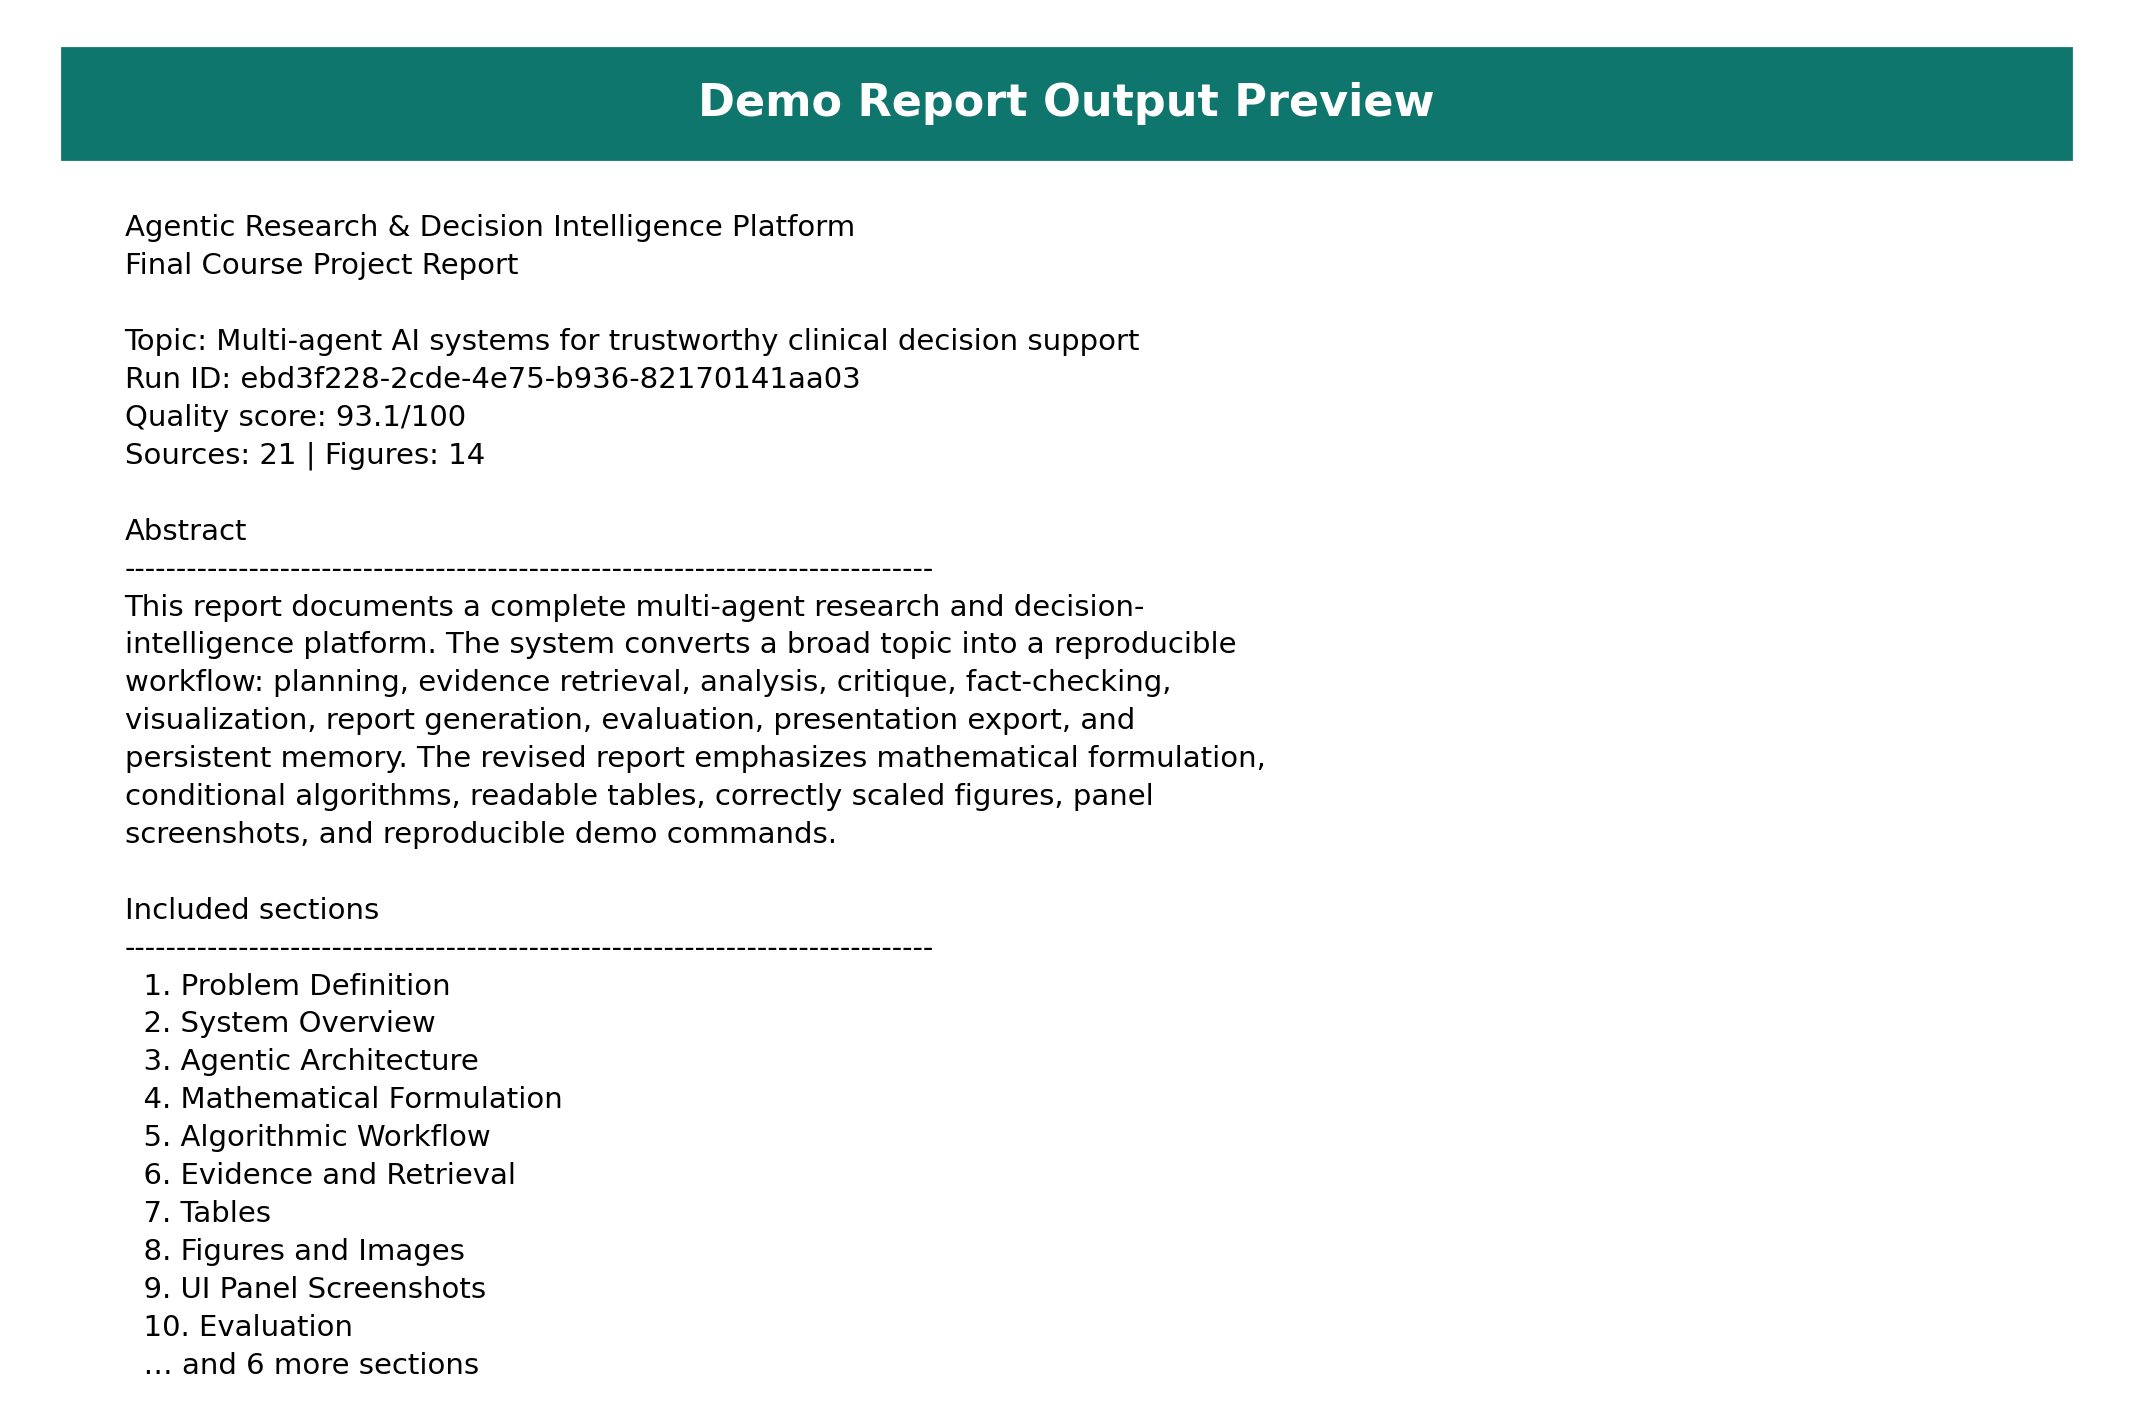
\includegraphics[width=0.95\linewidth,height=0.78\textheight,keepaspectratio]{assets/results/demo_report_output.png}
\caption{Demo report preview showing generated academic sections and run metadata.}
\label{fig:demo-report-preview}
\end{figure}
\FloatBarrier


\section{Report Generation and LaTeX Formatting}
The LaTeX generator now uses \texttt{tabularx}, an adaptive \texttt{Y} column type, \texttt{adjustbox}, smaller table padding, increased row spacing, and constrained figure dimensions. Inline math is preserved while regular text is escaped, so table cells can contain formulas such as $Q < \tau$ without being converted into broken text. Figures and screenshots use \texttt{keepaspectratio} with a maximum height, which prevents stretched diagrams and tiny unreadable page images.

\section{Evaluation Methodology}
The evaluator scores factuality, relevance, completeness, structure, citation quality, clarity, visual quality, and reproducibility. These dimensions are important because a research assistant should be graded on traceability and artifact quality, not just prose fluency. The final score in this run is 93.1/100.


\begin{table}[!htbp]
\centering
\caption{Final Evaluation Scores}
\label{tab:evaluation-scores}
\begingroup
\scriptsize
\setlength{\tabcolsep}{2.8pt}
\renewcommand{\arraystretch}{1.35}
\begin{adjustbox}{max width=\textwidth}
\begin{tabularx}{\textwidth}{@{}>{\RaggedRight\arraybackslash}p{0.20\textwidth}>{\RaggedRight\arraybackslash}p{0.11\textwidth}Y@{}}
\toprule
\textbf{Dimension} & \textbf{Score} & \textbf{Interpretation} \\
\midrule
Factuality & 96.0 & Groundedness and unsupported-claim control \\
Relevance & 90.0 & Alignment with the selected topic \\
Completeness & 92.0 & Coverage of required deliverables \\
Structure & 88.0 & Organization and readability \\
Citation quality & 95.0 & Evidence traceability \\
Clarity & 89.0 & Presentation quality \\
Visual quality & 100.0 & Figure and UI artifact quality \\
Reproducibility & 95.0 & Repeatable mock-mode execution \\
Total & 93.1 & Overall artifact score \\
\bottomrule
\end{tabularx}
\end{adjustbox}
\endgroup
\end{table}
\FloatBarrier


\section{Results}
The mock run completed with 21 sources, 14 figure records, a canonical LaTeX source, a compiled PDF, demo screenshots, result images, evaluation JSON/Markdown, and presentation output. The report is intentionally artifact-heavy: tables document agent behavior and API design; formulas document scoring; algorithms document control flow; figures document architecture and UI behavior.

\section{Claim Checks}
\begin{itemize}
\item \textbf{Supported}: Retrieval grounding can reduce unsupported generation by forcing reports to cite external evidence. ((Patrick Lewis, 2020), (Shahul Es, 2023)). Supported by tagged source evidence.
\item \textbf{Supported}: Clinical decision support requires human oversight and careful workflow integration. ((Amit X. Garg, 2005), (Kensaku Kawamoto, 2005), (Reed T. Sutton, 2020)). Supported by tagged source evidence.
\item \textbf{Supported}: Conditional multi-agent graphs make critique and revision loops explicit. ((Google, 2026), (Qingyun Wu, 2023), (Shunyu Yao, 2022)). Supported by tagged source evidence.
\item \textbf{Supported}: Evaluation should include factuality, relevance, structure, citation quality, and reproducibility. ((Amit X. Garg, 2005), (Brennan Vasey, 2022), (Kensaku Kawamoto, 2005)). Supported by tagged source evidence.
\item \textbf{Supported}: The prototype is not a medical device and should not produce patient-specific diagnosis. ((Brennan Vasey, 2022), (Reed T. Sutton, 2020), (World Health Organization, 2021)). Supported by tagged source evidence.
\end{itemize}

\section{Critic Notes}
\begin{itemize}
\item Evidence coverage is adequate for a prototype, but deployment claims must remain bounded.
\item The system should emphasize clinician oversight, auditability, and uncertainty rather than autonomous diagnosis.
\item The mock corpus is suitable for reproducible testing but must be refreshed for real clinical use.
\end{itemize}

\section{Error Analysis}
Expected errors include stale sources, unsupported claims, shallow critique, malformed citations, and broken rendering. The system mitigates these through deterministic retrieval, explicit critic notes, citation gating, evaluation thresholds, generated screenshots, and a render-and-check PDF workflow. For production, passage-level entailment and source freshness checks should be added before any high-stakes deployment.

\section{Ethical and Safety Considerations}
The clinical scenario is used only as a demanding research context. The system must not be used for diagnosis or treatment. Real deployment would require privacy controls, audit logs, security review, institution-approved source corpora, clinician accountability, bias evaluation, and human approval gates. The report therefore frames clinical decision support as a governance and workflow problem, not merely a model-quality problem.

\section{Testing and Reproducibility}
The project can be regenerated with the commands below. Mock mode is the grading default because it produces repeatable evidence, figures, screenshots, evaluation files, and reports.
\begin{lstlisting}[caption={Local verification commands}]
python -m venv .venv
source .venv/bin/activate
pip install -r requirements.txt
export USE_MOCK_LLM=true
python scripts/capture_ui_screenshots.py
python scripts/generate_latex_report.py
python scripts/build_report_pdf.py
pytest
\end{lstlisting}

\section{Limitations}
The current corpus is static, the fact checker is metadata-level rather than entailment-level, and the evaluator uses deterministic heuristics. The UI is intended for demonstration rather than production operations. These limitations are acceptable for a final project because they make grading reproducible, but they must be addressed before real deployment.

\section{Future Work}
Future work should add live retrieval adapters, vector search over approved corpora, stronger natural-language entailment, asynchronous job queues, authentication, richer audit trails, human review checkpoints, and benchmarking against clinical reporting standards. The architecture already isolates these improvements behind agent and tool contracts.

\section{Conclusion}
The platform demonstrates a complete, reproducible, and inspectable agentic research workflow. The updated LaTeX generator produces a fuller academic report with robust tables, preserved mathematical notation, explicit algorithms, constrained figures, refreshed UI screenshots, and clearer explanations of how the multi-agent system works.

\nocite{*}
\bibliographystyle{plain}
\bibliography{references}
\end{document}
